\documentclass[compress]{beamer}
\usepackage[ngerman]{babel}
\usepackage{graphicx}
\usepackage{subfiles}
\usepackage{listings}

\graphicspath{{images/}}

% \setbeameroption{show notes}

\usetheme[noflama]{custom}

\title{Virtualisierte Arbeitsumgebung für den Test verteilter Systeme}
\subtitle{Microservice-Architektur mit Docker, Clojure \& Elm}
\author{Jan-Philipp Willem}
\institute{Fakultät für Informatik\\Hochschule Mannheim}
\date{13. Dezember 2017}

\begin{document}

% \begin{frame}[noframenumbering,plain]
% \end{frame}

\maketitle

% \begin{frame}[noframenumbering,plain]{Project-Repository}
% \includegraphics[width=0.8\textwidth]{google.pdf}
% \end{frame}

\section*{Gliederung}
\begin{frame}[noframenumbering,plain]{Gliederung}
  \tableofcontents[hideallsubsections]
  →~{\color{orange}\url{https://github.com/jwillem/var-tool}}
\end{frame}

\section{Anforderungen}
% \begin{frame}{Bisheriger Ablauf}
%   \begin{itemize}
%     \item Student soll (verteilte) Aufgaben programmieren
%     \item Es wird die Benutzung von schwergewichtigen IDEs vorgeschlagen
%     \item Eclipse, Netbeans bieten Integrationen zu diversen Servern/Technologien
%     \item Funktionsweise kann in gegebener (Dev-)Umgebung getestet werden
%   \end{itemize}
%   \begin{itemize}
%     \item Gefahr: keine echte Verteilung
%     \item Umgebung verschieden zu Production
%     \item Ergebnis kann sich erheblich unterscheiden (Seiteneffekte,..)
%     \item Einrichtung der Dev-Umgebung kann dennoch schwierig sein
%   \end{itemize}
% \end{frame}
\begin{frame}{Anforderungen (1/2)}
  \begin{itemize}
    \item Dozent beschreibt ein Experiment im Kontext von verteilten Systemen
    \item Feste Anzahl an Instanzen, auf denen Lösungen von Programmieraufgaben ausgeführt werden sollen
    \item Benötigte Technologien können dabei auch definiert werden
    \item Pro Instanz: Angabe von Name, Ports, standard Command
    \item Getrennte Netzwerke zwischen Experimenten
  \end{itemize}
\end{frame}
\begin{frame}{Anforderungen (2/2)}
  \begin{itemize}
    \item Studenten sollen mithilfe der Experimente gewisse Aufgaben lösen
    \item Upload von Programmpaketen im Frontend
    \item Angabe von Main-Class und Argumentenliste
    \item Einzelnes Starten der Instanzen
    \item Eingabe im Frontend führt zu Ereignis bei stdin von Instanz
    \item Geschehene Logs (stdout, stderror) in Instanz führen zu Ereignis im Frontend
  \end{itemize}
\end{frame}
% \begin{frame}{Erhoffte Vorteile}
%   \begin{itemize}
%     \item Dev-Umgebung zum Starten der Instanzen muss nicht zwingend eingerichtet werden
%     \item Konsistentes UI des Tools zwischen Aufgaben \break (\& Vorlesungen?)
%     \item Durch Hochladen der Programmpakete pro Instanz wird Verteilung auf Netzwerkebene (hoffentlich) besser wahrgenommen
%     \item Hostnamen der Instanzen nicht localhost
%   \end{itemize}
% \end{frame}

\section{Technologien}
\begin{frame}{Docker}
  \begin{columns}[c]
    \column{.7\textwidth}
  \begin{itemize}
    \item Software zum Deployment von Applikationen innerhalb von Containern
    \item Ähnelt Vorgehensweise von Virtuellen Maschinen
    \item Im Gegensatz: Mithilfe von Docker-\break Daemon laufen Prozesse direkt auf Host-OS
    % \item Dennoch isoliert (CGroups, Kernel Namespaces, SELinux, AppArmor,..)
    \item Keine spezifische Hardware-\break Infrastruktur vorgeschrieben
    % \item Beste Unterstützung durch Linux-Derivat (Kernel-Tricks)
    \item Lauffähig auf Linux, Mac-OS, Windows
  \end{itemize}
    \column{.3\textwidth}
    
\includegraphics[width=80pt]{docker_logo.png}
  \end{columns}
\end{frame}
% \begin{frame}{Container}
%   \begin{itemize}
%     \item Deskriptive \& triviale Beschreibung eines Systems und dessen Bestandteile (Rezept)
%     \item Instruktionen um Abhähigkeiten zu installieren, Konfigurationen vorzunehmen und Build-Steps auszuführen
%     \item Kein Transferieren von großen Builds nötig, da Image durch Dockerfile erzeugbar
%     \item Granulare Sub-Images
    % \item Trägt implizit zur Dokumentation bei: Jede Änderung an einem Container muss im Rezept ergänzt werden!
%   \end{itemize}
% \end{frame}

\begin{frame}{Clojure}
  \begin{columns}[c]
    \column{.7\textwidth}
    \begin{itemize}
      \item Moderner Lisp-Dialekt auf JVM
      \item Fokus liegt auf funktionalem Paradigma
      \item dynamisch typisiert
      \item Datenstrukturen sind Immutable
      \item Interessantes Konzept der Nebenläufigkeit: Communicating Sequential Processes (CSP)
      \item Interoperabilität zu JAVA
    \end{itemize}
    \column{.3\textwidth}
    
\includegraphics[width=80pt]{clojure_logo.png}
  \end{columns}
\end{frame}

\begin{frame}{Elm}
  \begin{columns}[c]
    \column{.7\textwidth}
    \begin{itemize}
      \item Rein funktionale Sprache
      \item ML-artig, ähnlich zu bspw. Haskell
      \item Kompiliert zu Java-Script
      \item DSL für HTML, SVG
      \item Sinnvolle Abstraktionen wie bspw. von Websockets
      \item Virtual DOM, ähnlich zu React
      \item Statisch typisiert, dabei sehr hilfreicher Compiler \href{http://elm-lang.org/blog/compiler-errors-for-humans}{\color{orange}+}
      \item Kein NULL oder undefined
      \item Core-API nutzt bei unsicheren Werten die Monaden Maybe oder Result \href{https://guide.elm-lang.org/error_handling/maybe.html}{\color{orange}+}
      \item The-Elm-Architecture (TEA), Ursprung von Redux in JS \href{https://guide.elm-lang.org/architecture/}{\color{orange}+}
    \end{itemize}
    \column{.3\textwidth}
    
\includegraphics[width=80pt]{elm_logo.png}
  \end{columns}
\end{frame}

% \begin{frame}{Dockerfile}
%   \AddToShipoutPictureFG*{%
%     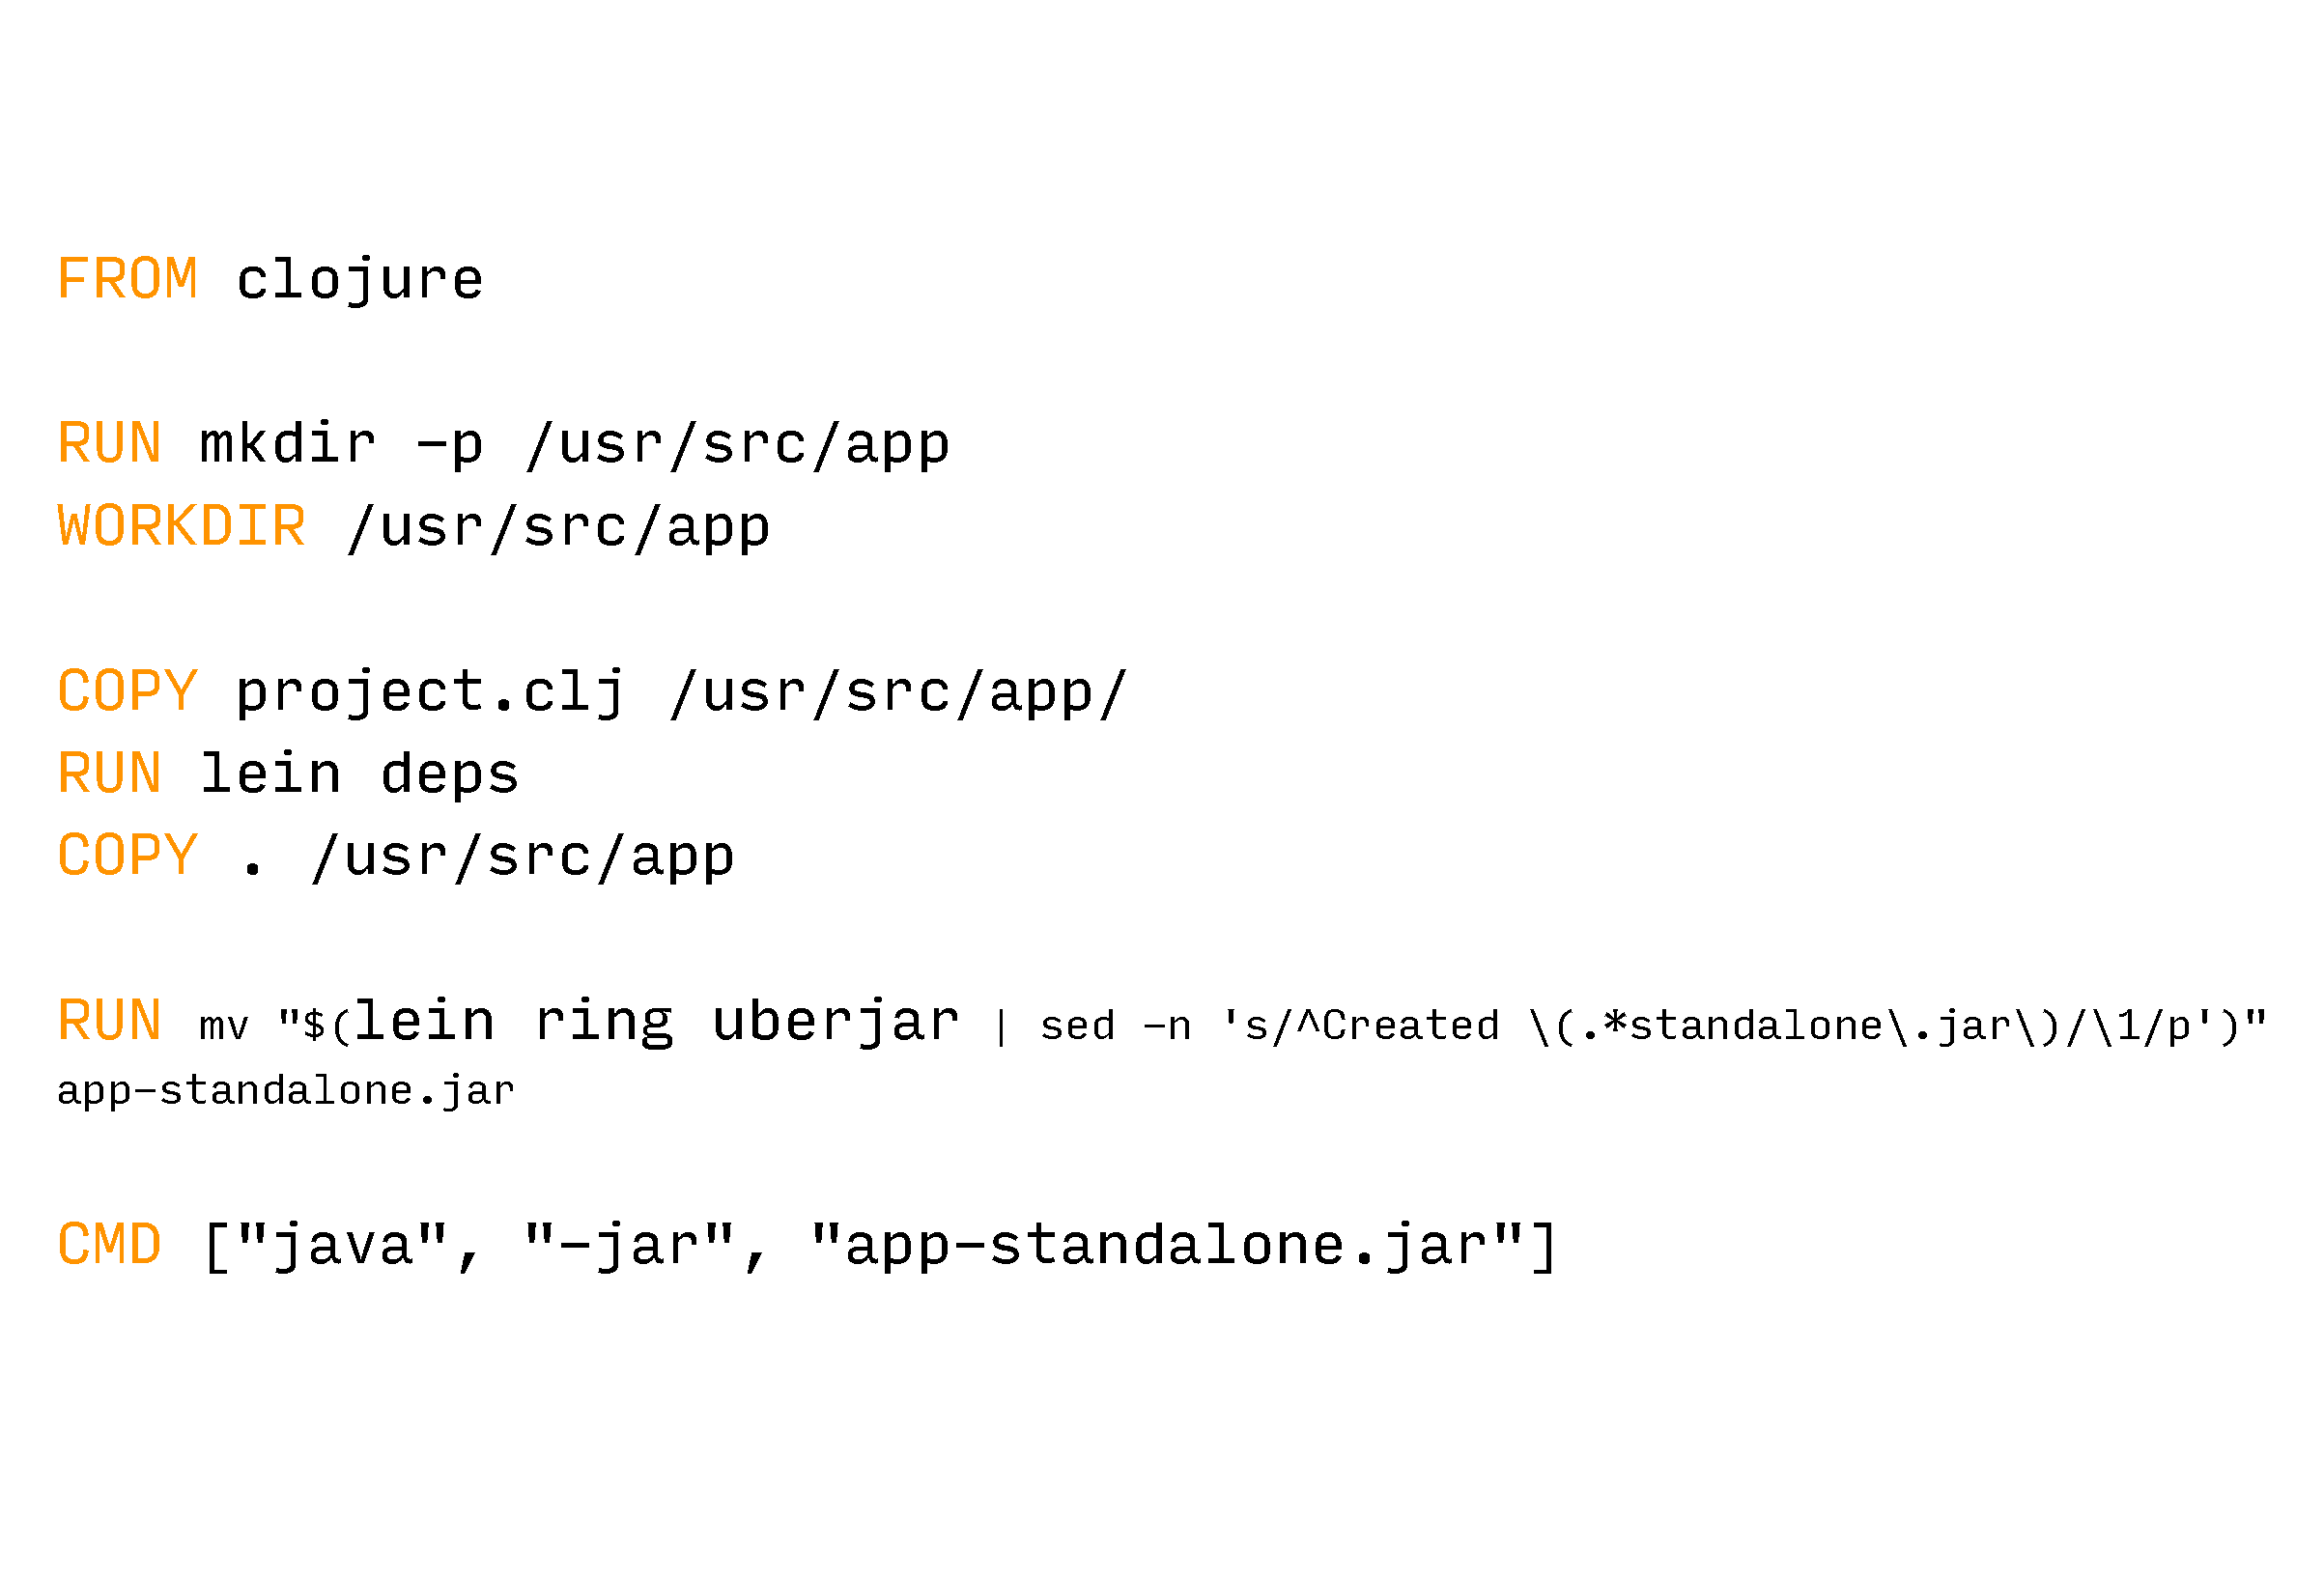
\includegraphics[width=\paperwidth,height=\textheight]{dockerfile.pdf}
%   }
% \end{frame}

% \begin{frame}{Docker-Compose}
%   \begin{itemize}
%     \item Tool zur Unterstützung von Docker-Cli
%     \item Definition von Services als Bestandteil einer App
%     \item Ergänzende Angabe von Konfigurations-Parametern an Containern: Volume-Mounts, Ports, Env-Vars, Netzwerke,..
%     \item Muss sonst bei \texttt{docker exec} Command angegeben werden
%     \item Getrennte Environments für Dev, Test, Prod: \texttt{docker-compose[.dev].yml}
%     \item Zentrale Dokumentation!
%   \end{itemize}
% \end{frame}

\section{Inspiration}
\begin{frame}{Tmux Panes}

  % \AddToShipoutPictureFG*{%
  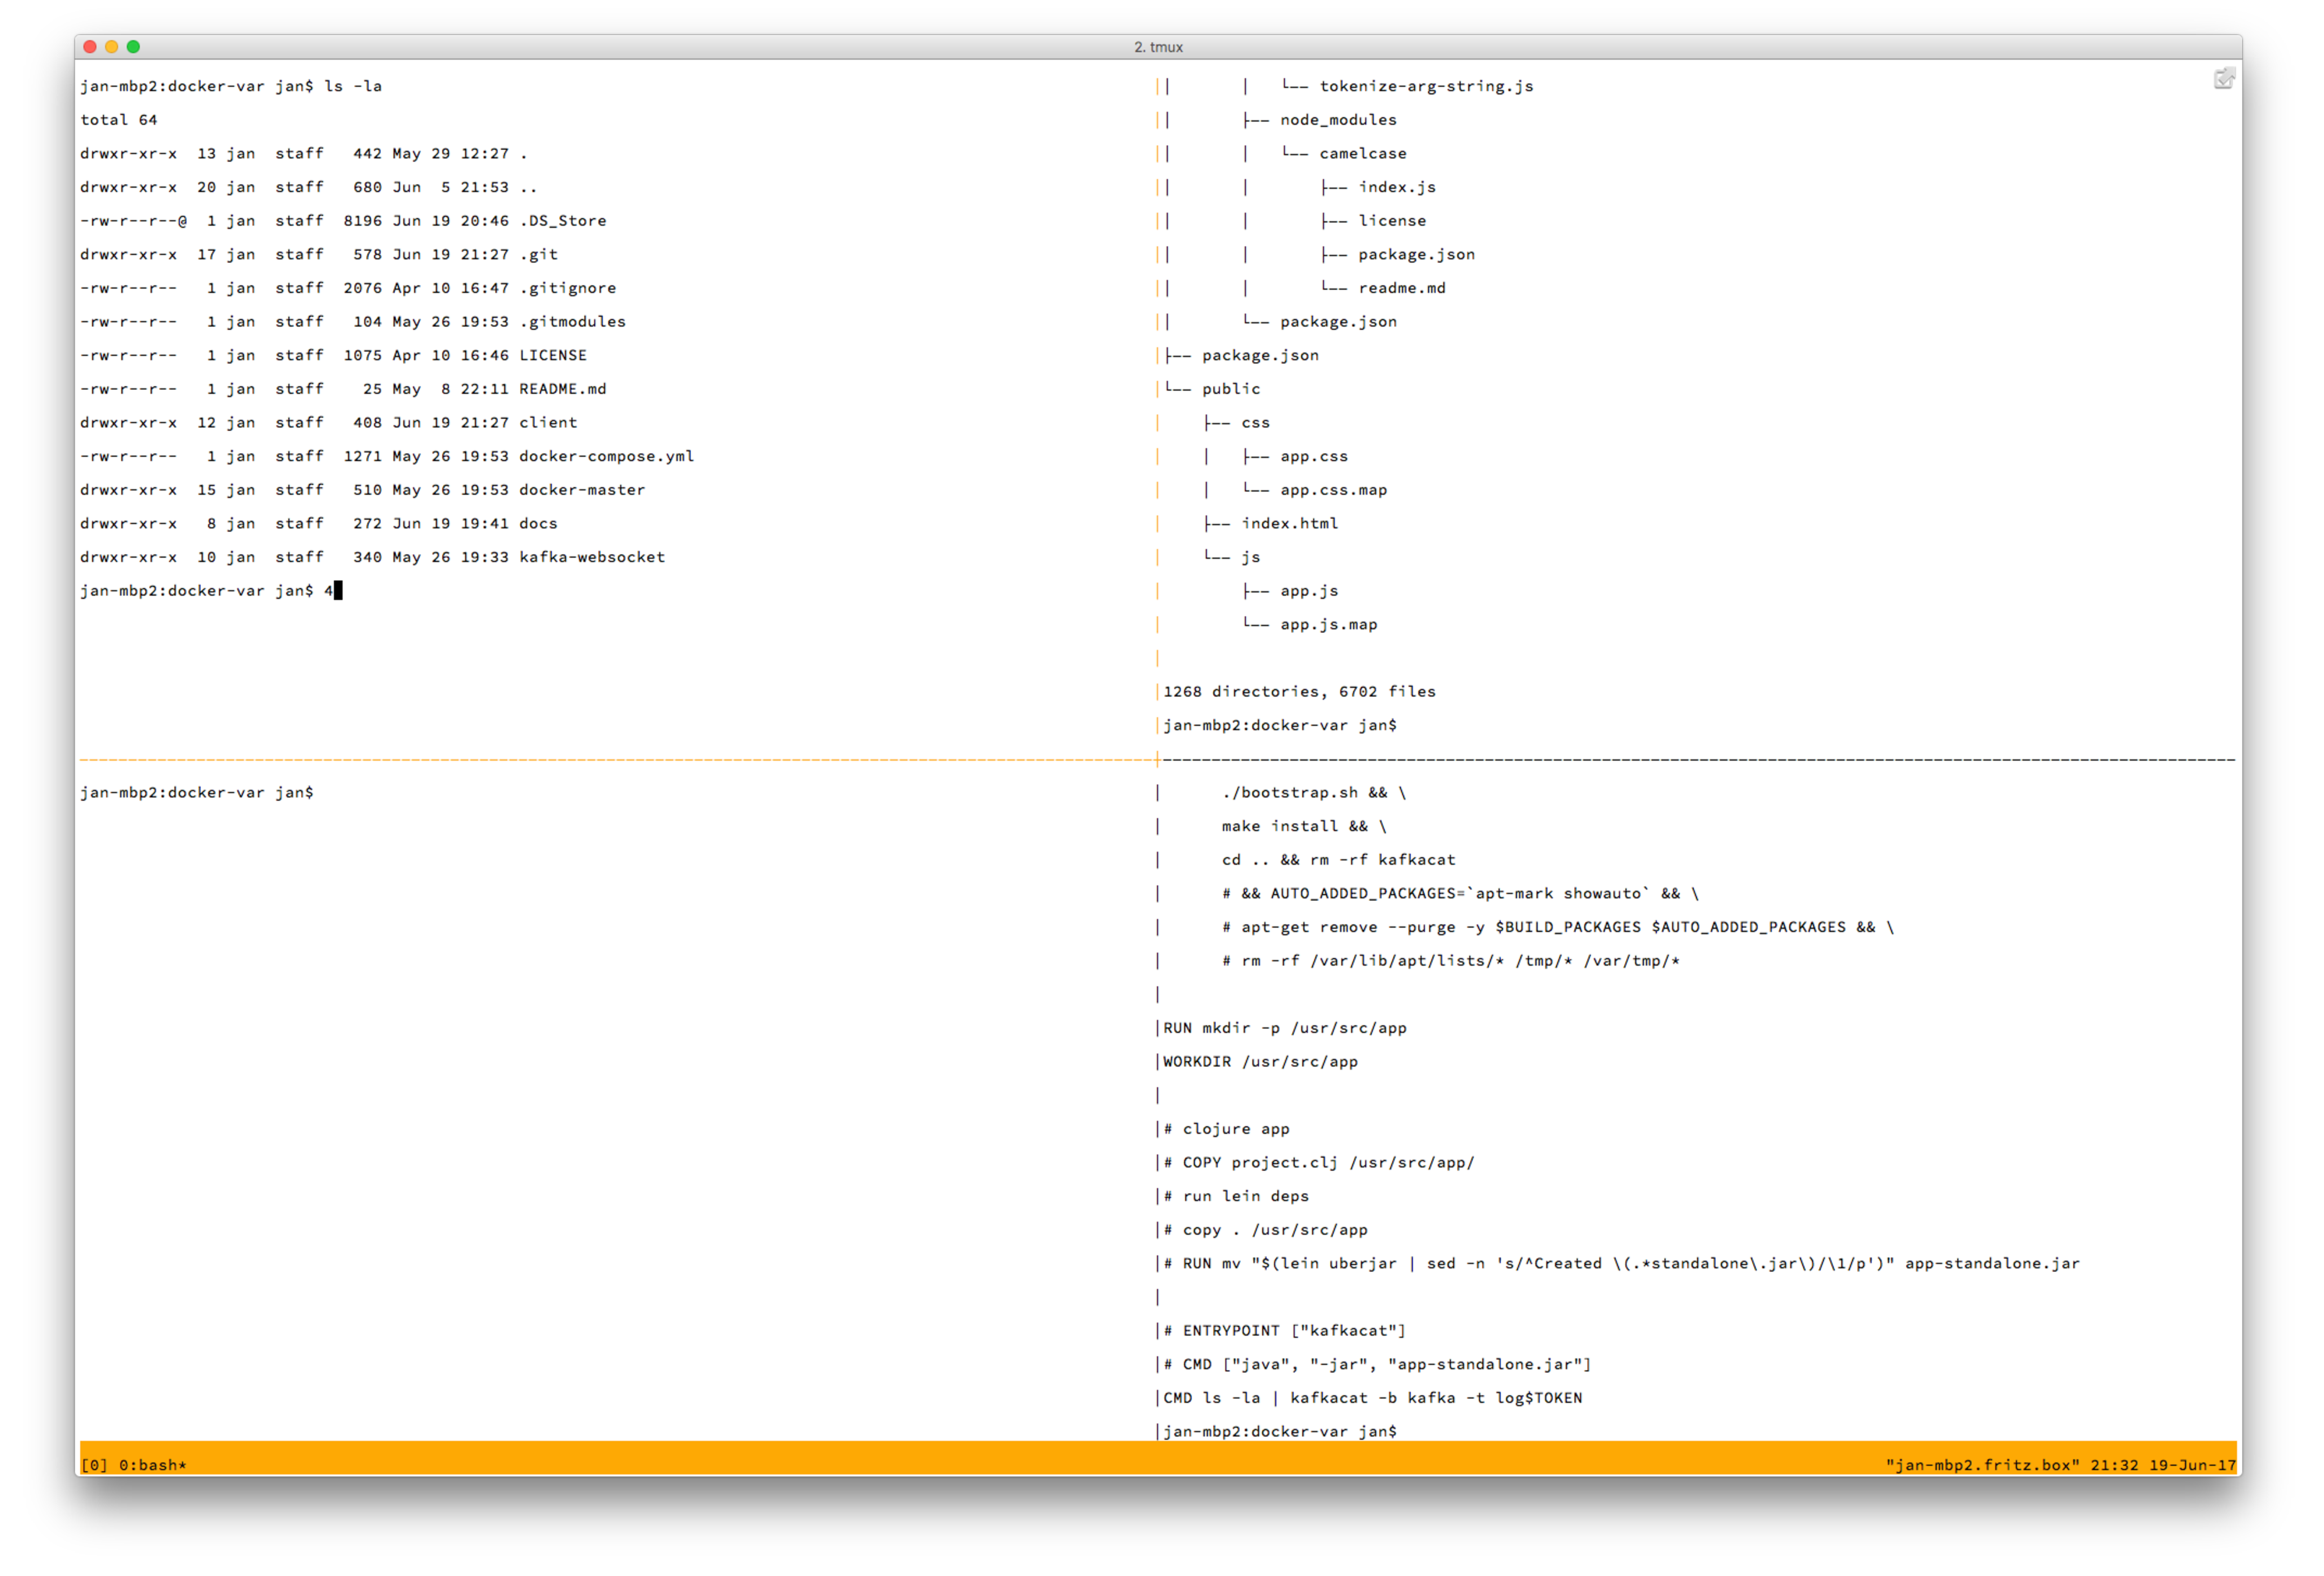
\includegraphics[width=\textwidth]{tmux.pdf}
  % }
\end{frame}
% \begin{frame}{Cloud-IDEs}
%   \begin{columns}
%     \column{.5\textwidth}
%     \begin{itemize}
%       \item Cloud 9
%       \item Source Lair
%       \item Eclipse Che
%       \item ...
%     \end{itemize}
%
%     \column{.5\textwidth}
%     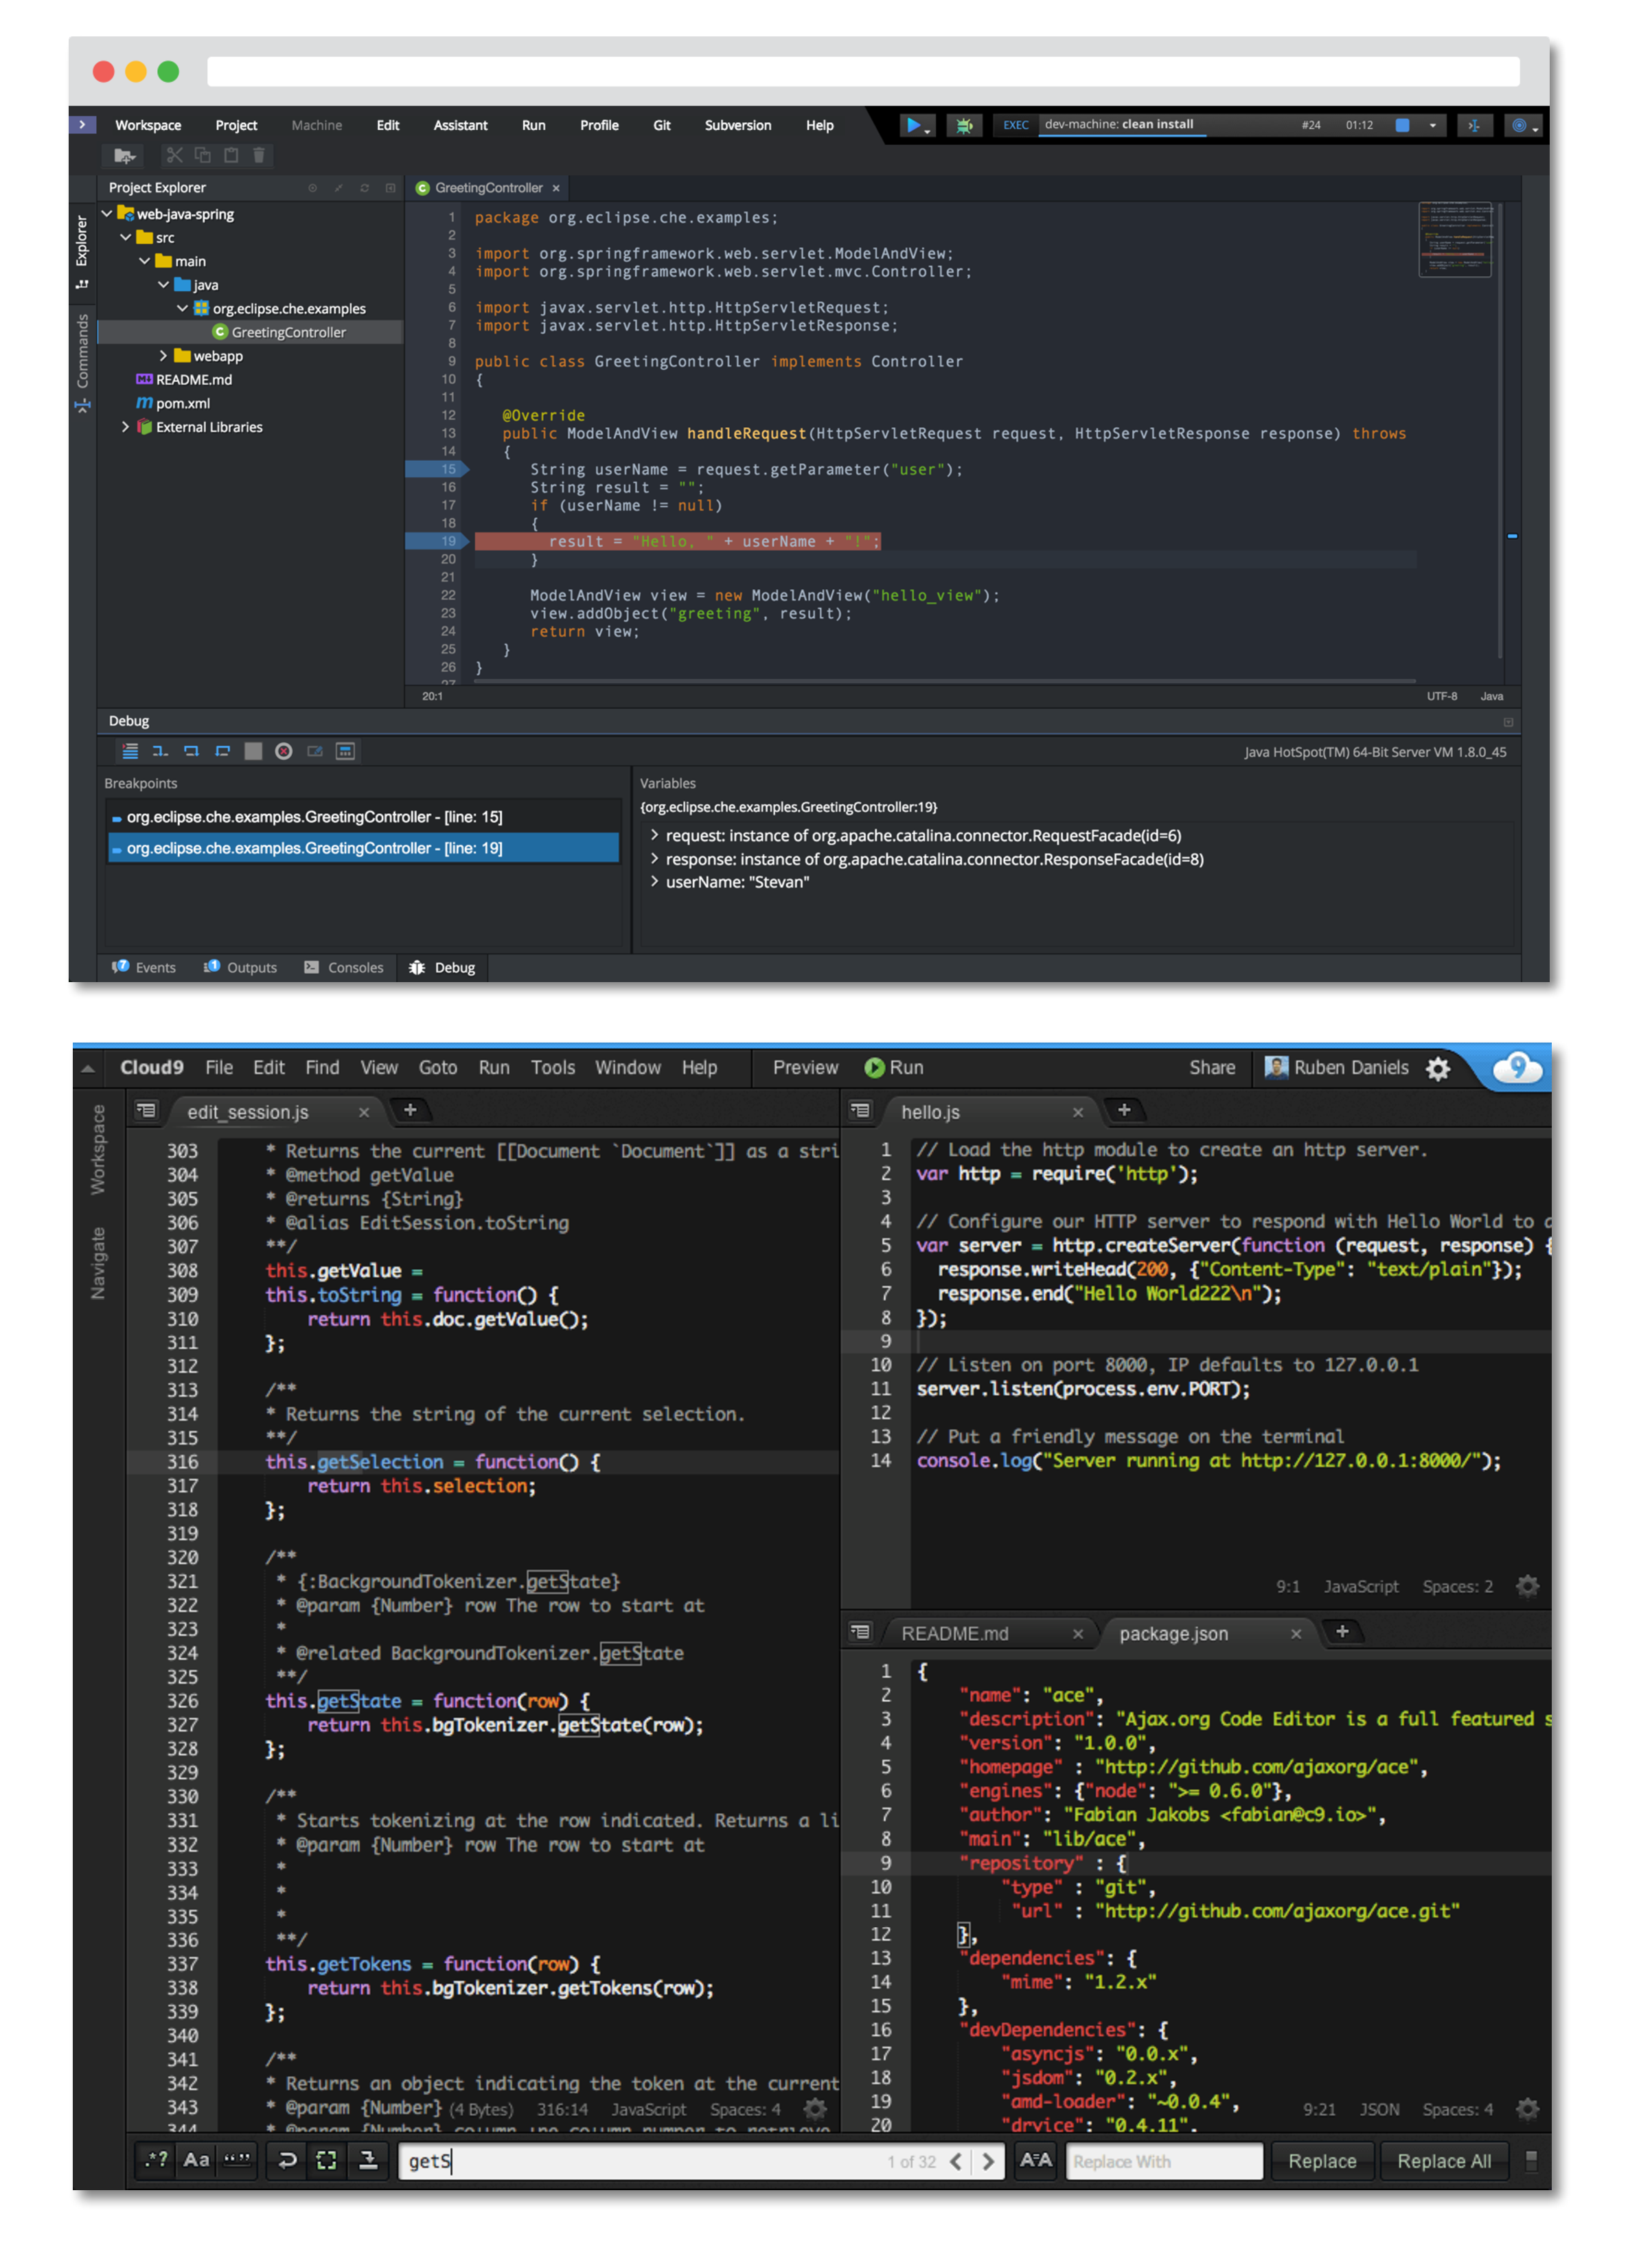
\includegraphics[width=\textwidth]{eclipse.pdf}
%   \end{columns}
% \end{frame}
% \begin{frame}{xterm.js}
%   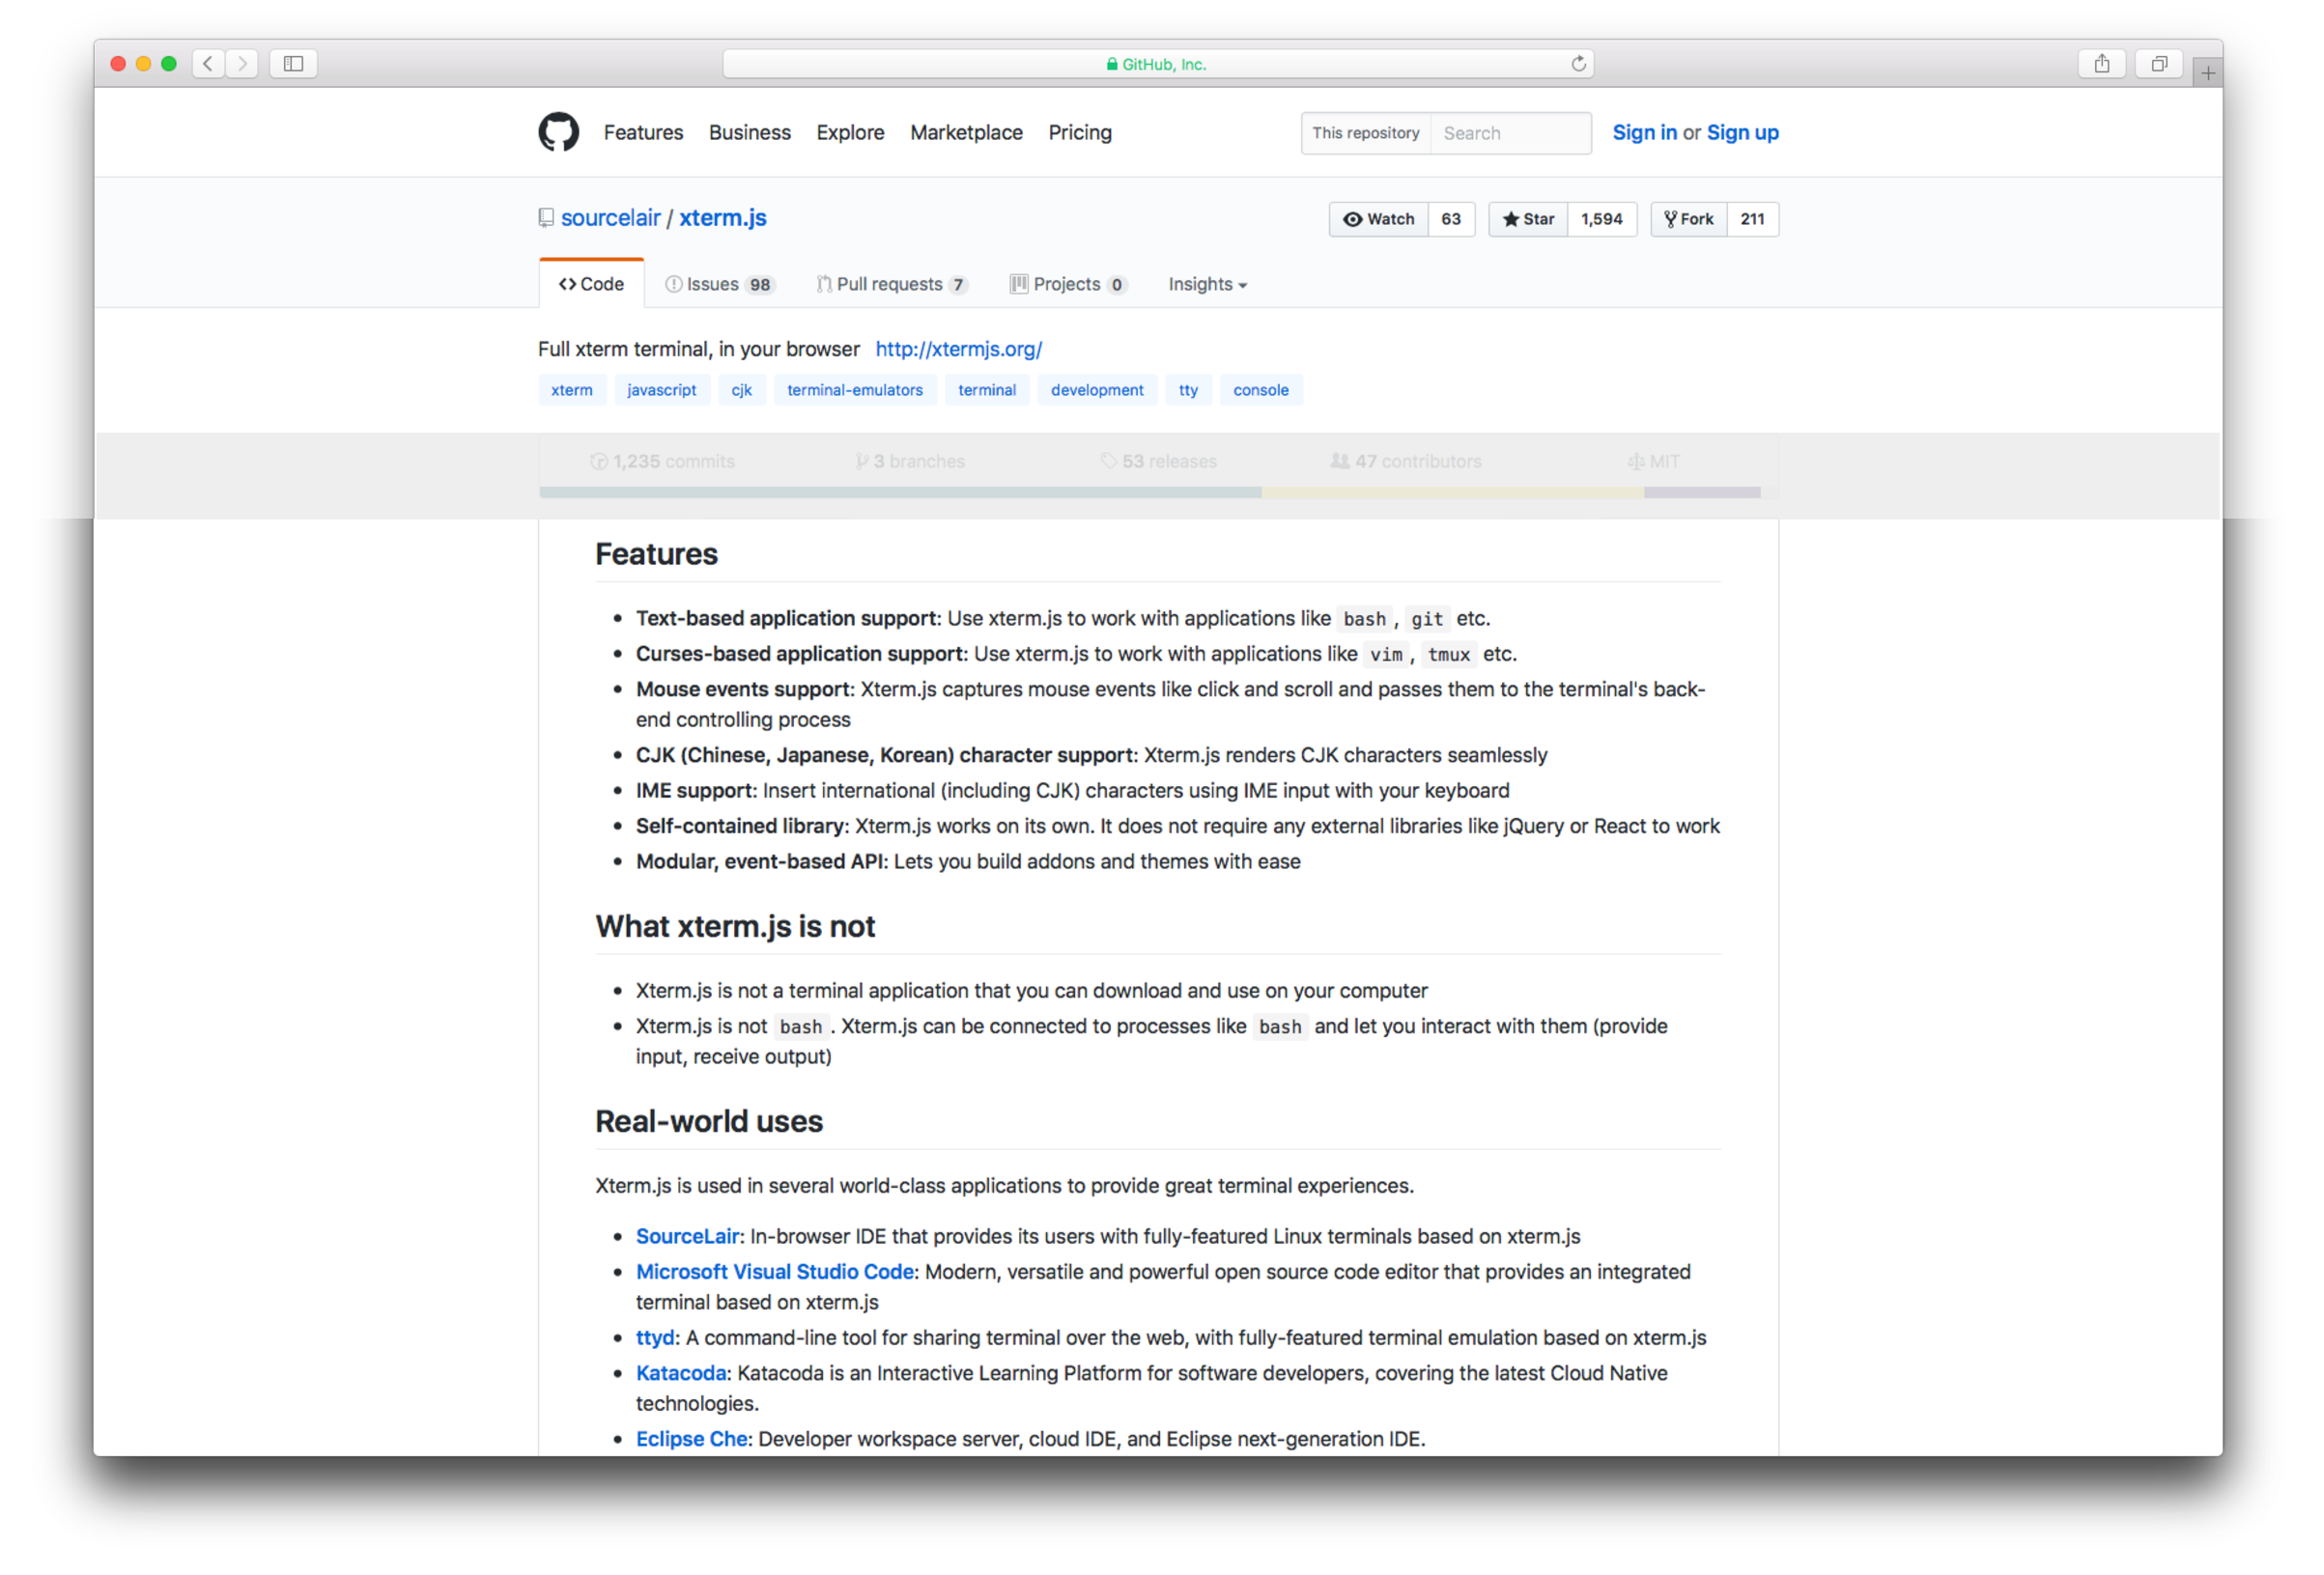
\includegraphics[width=\textwidth]{xterm.pdf}
% \end{frame}
\begin{frame}{ttyd}
  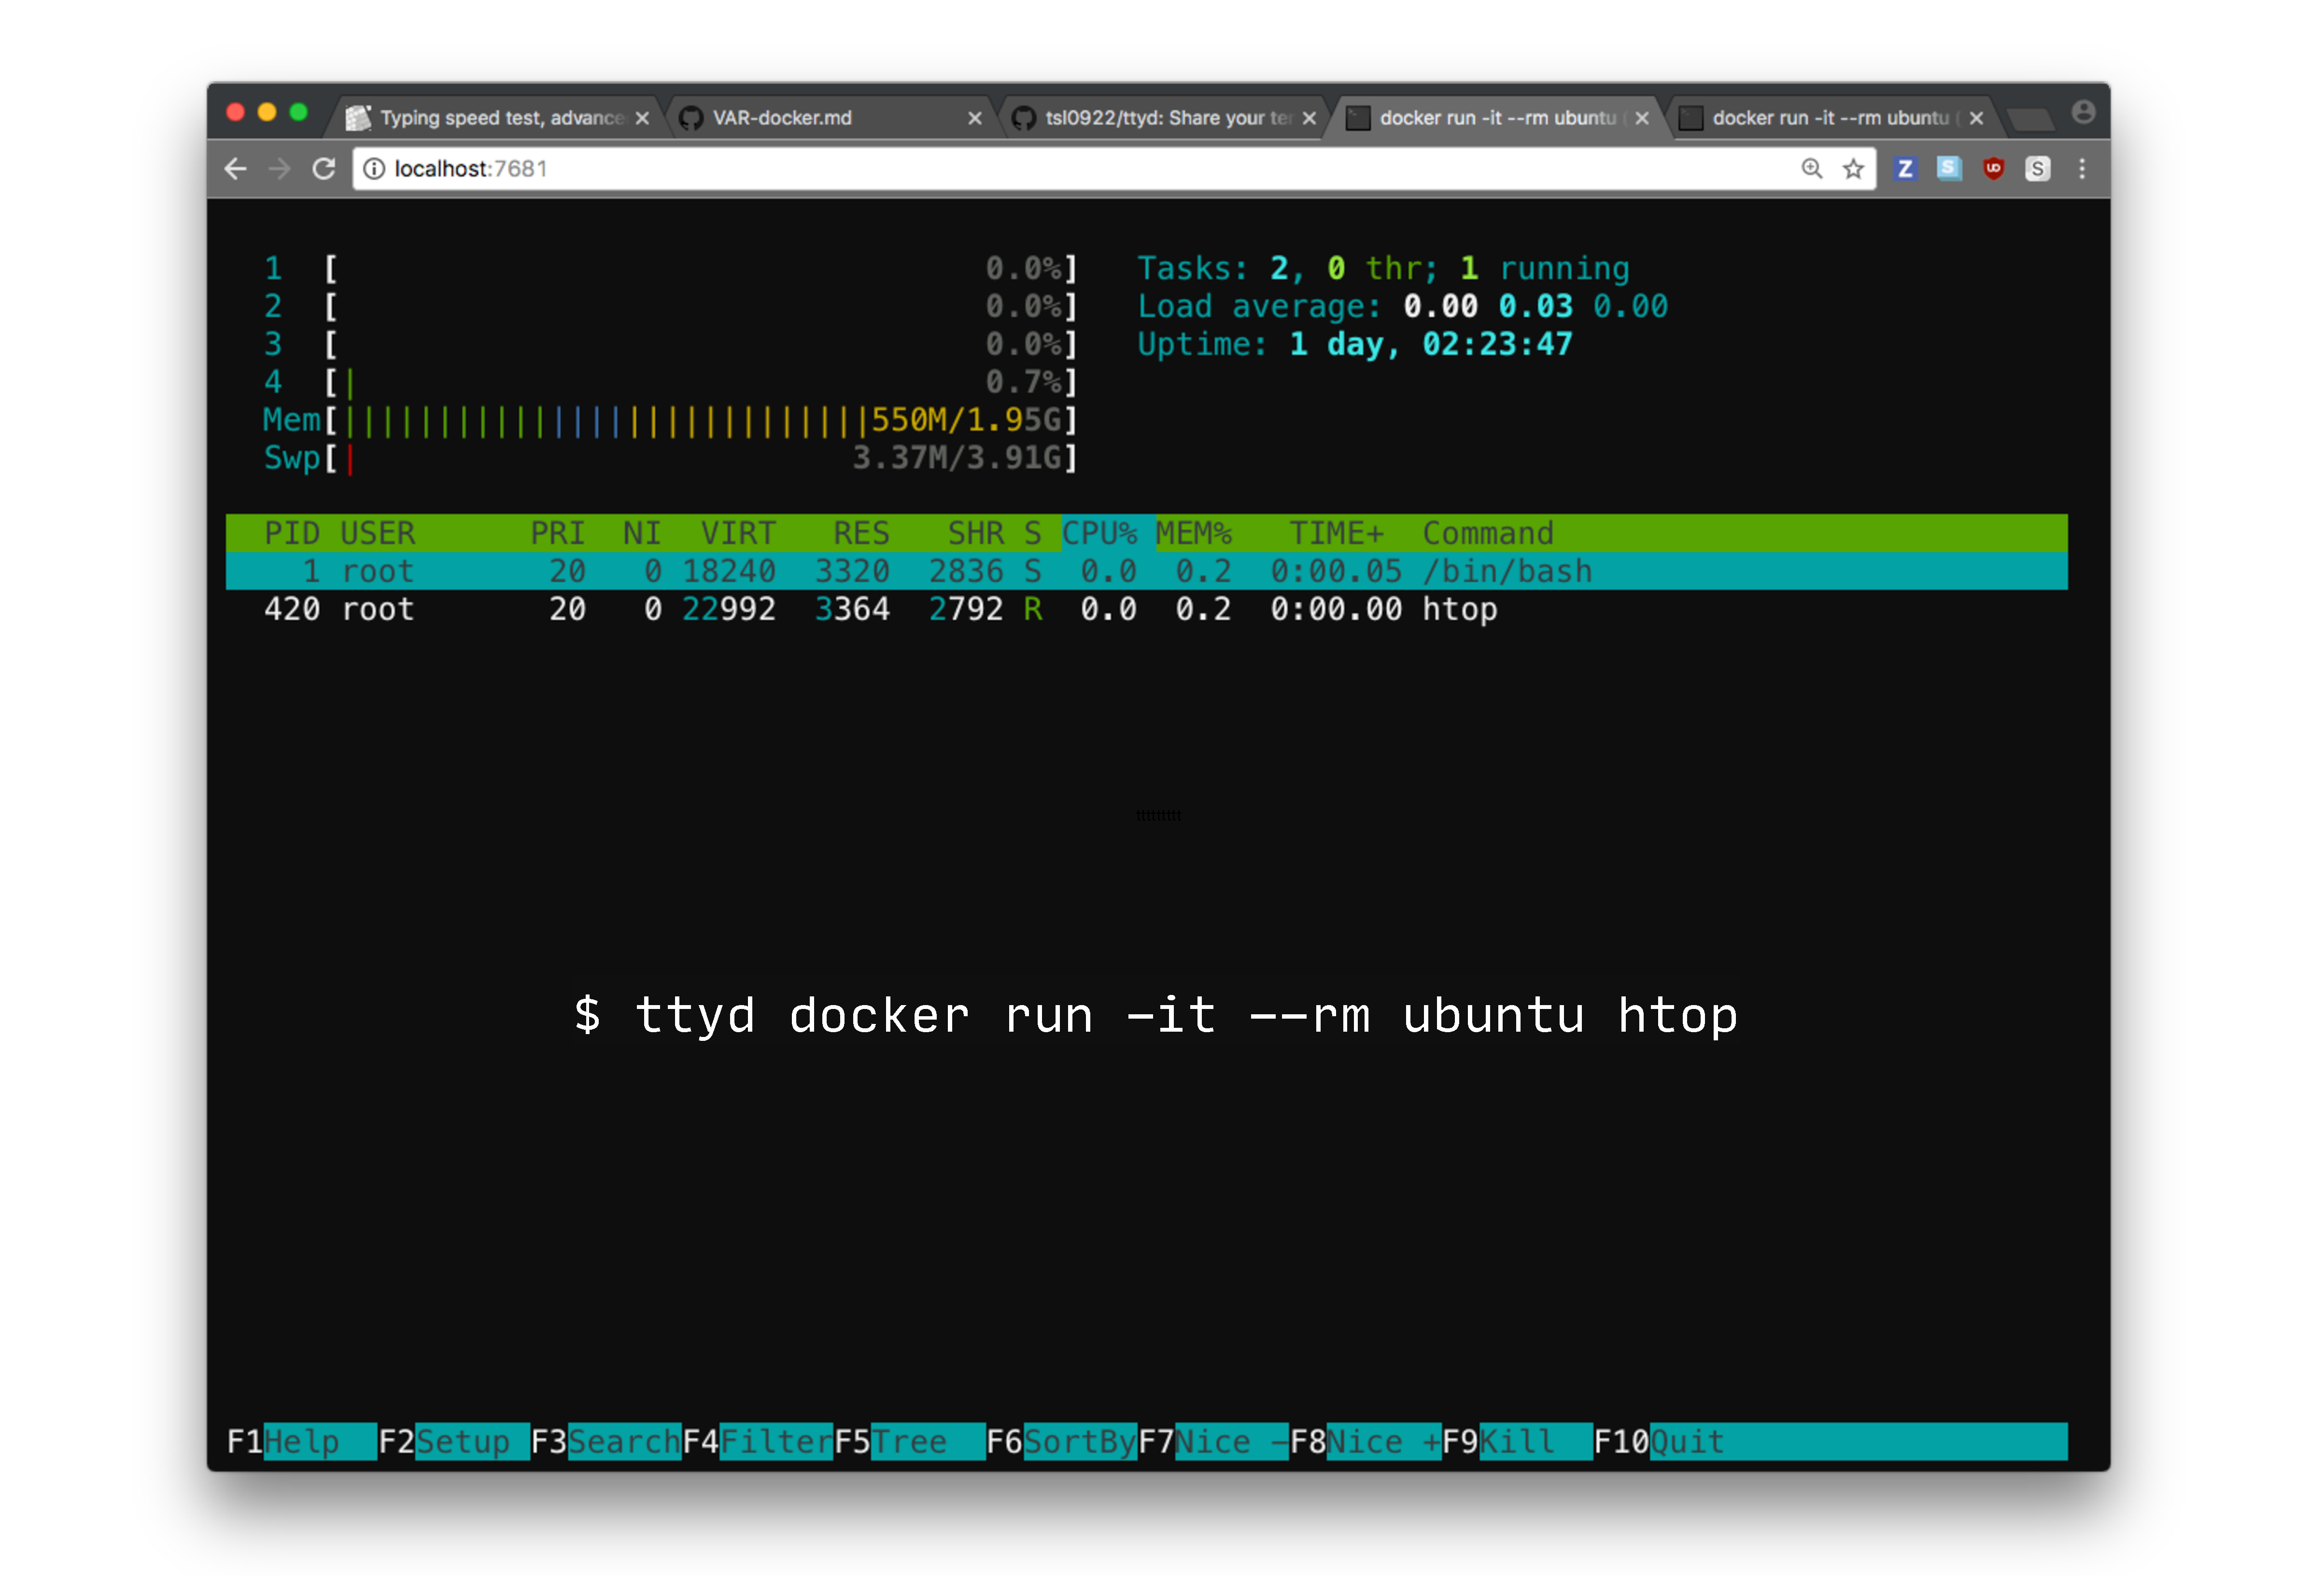
\includegraphics[width=\textwidth]{ttyd.pdf}
\end{frame}

\section{„VAR-Tool“}
% \begin{frame}{}
%   \AddToShipoutPictureFG*{%
%     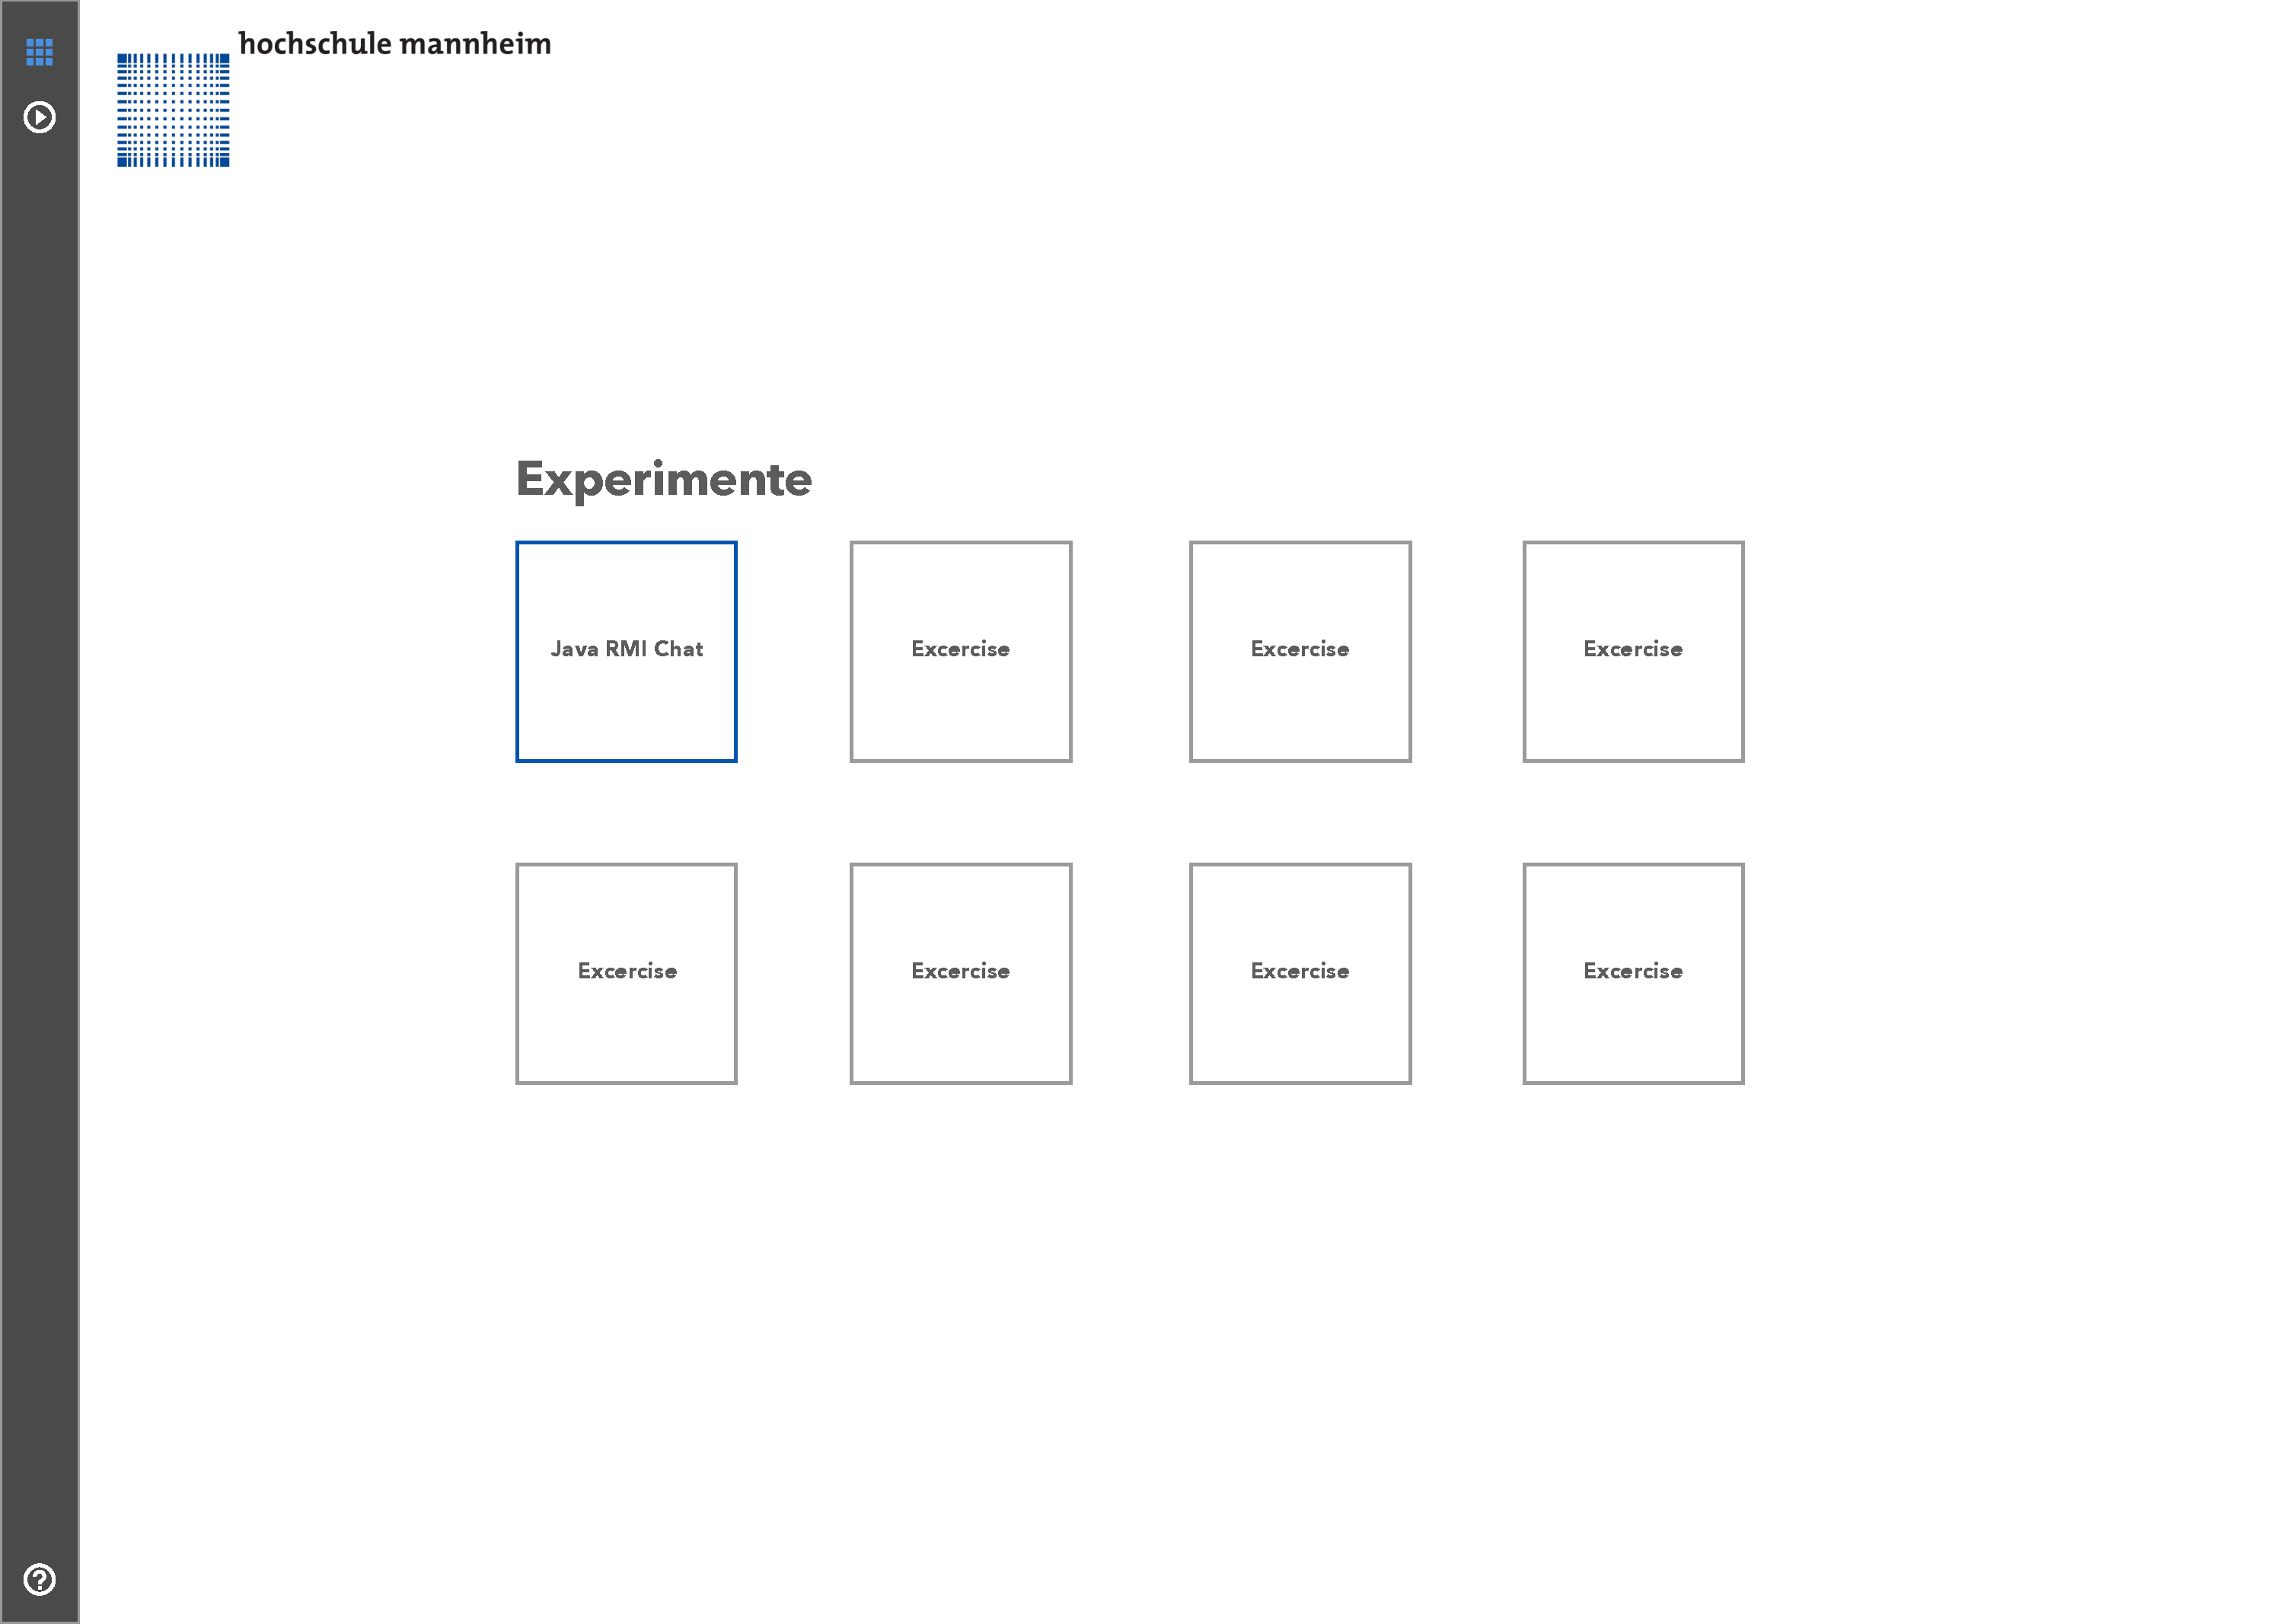
\includegraphics[width=\paperwidth,height=\paperheight,page=1]{ui-mockup.pdf}
%   }
% \end{frame}
% \begin{frame}{}
%   \AddToShipoutPictureFG*{%
%     \includegraphics[width=\paperwidth,height=\paperheight,page=2]{ui-mockup.pdf}
%   }
% \end{frame}
\begin{frame}{Network}
  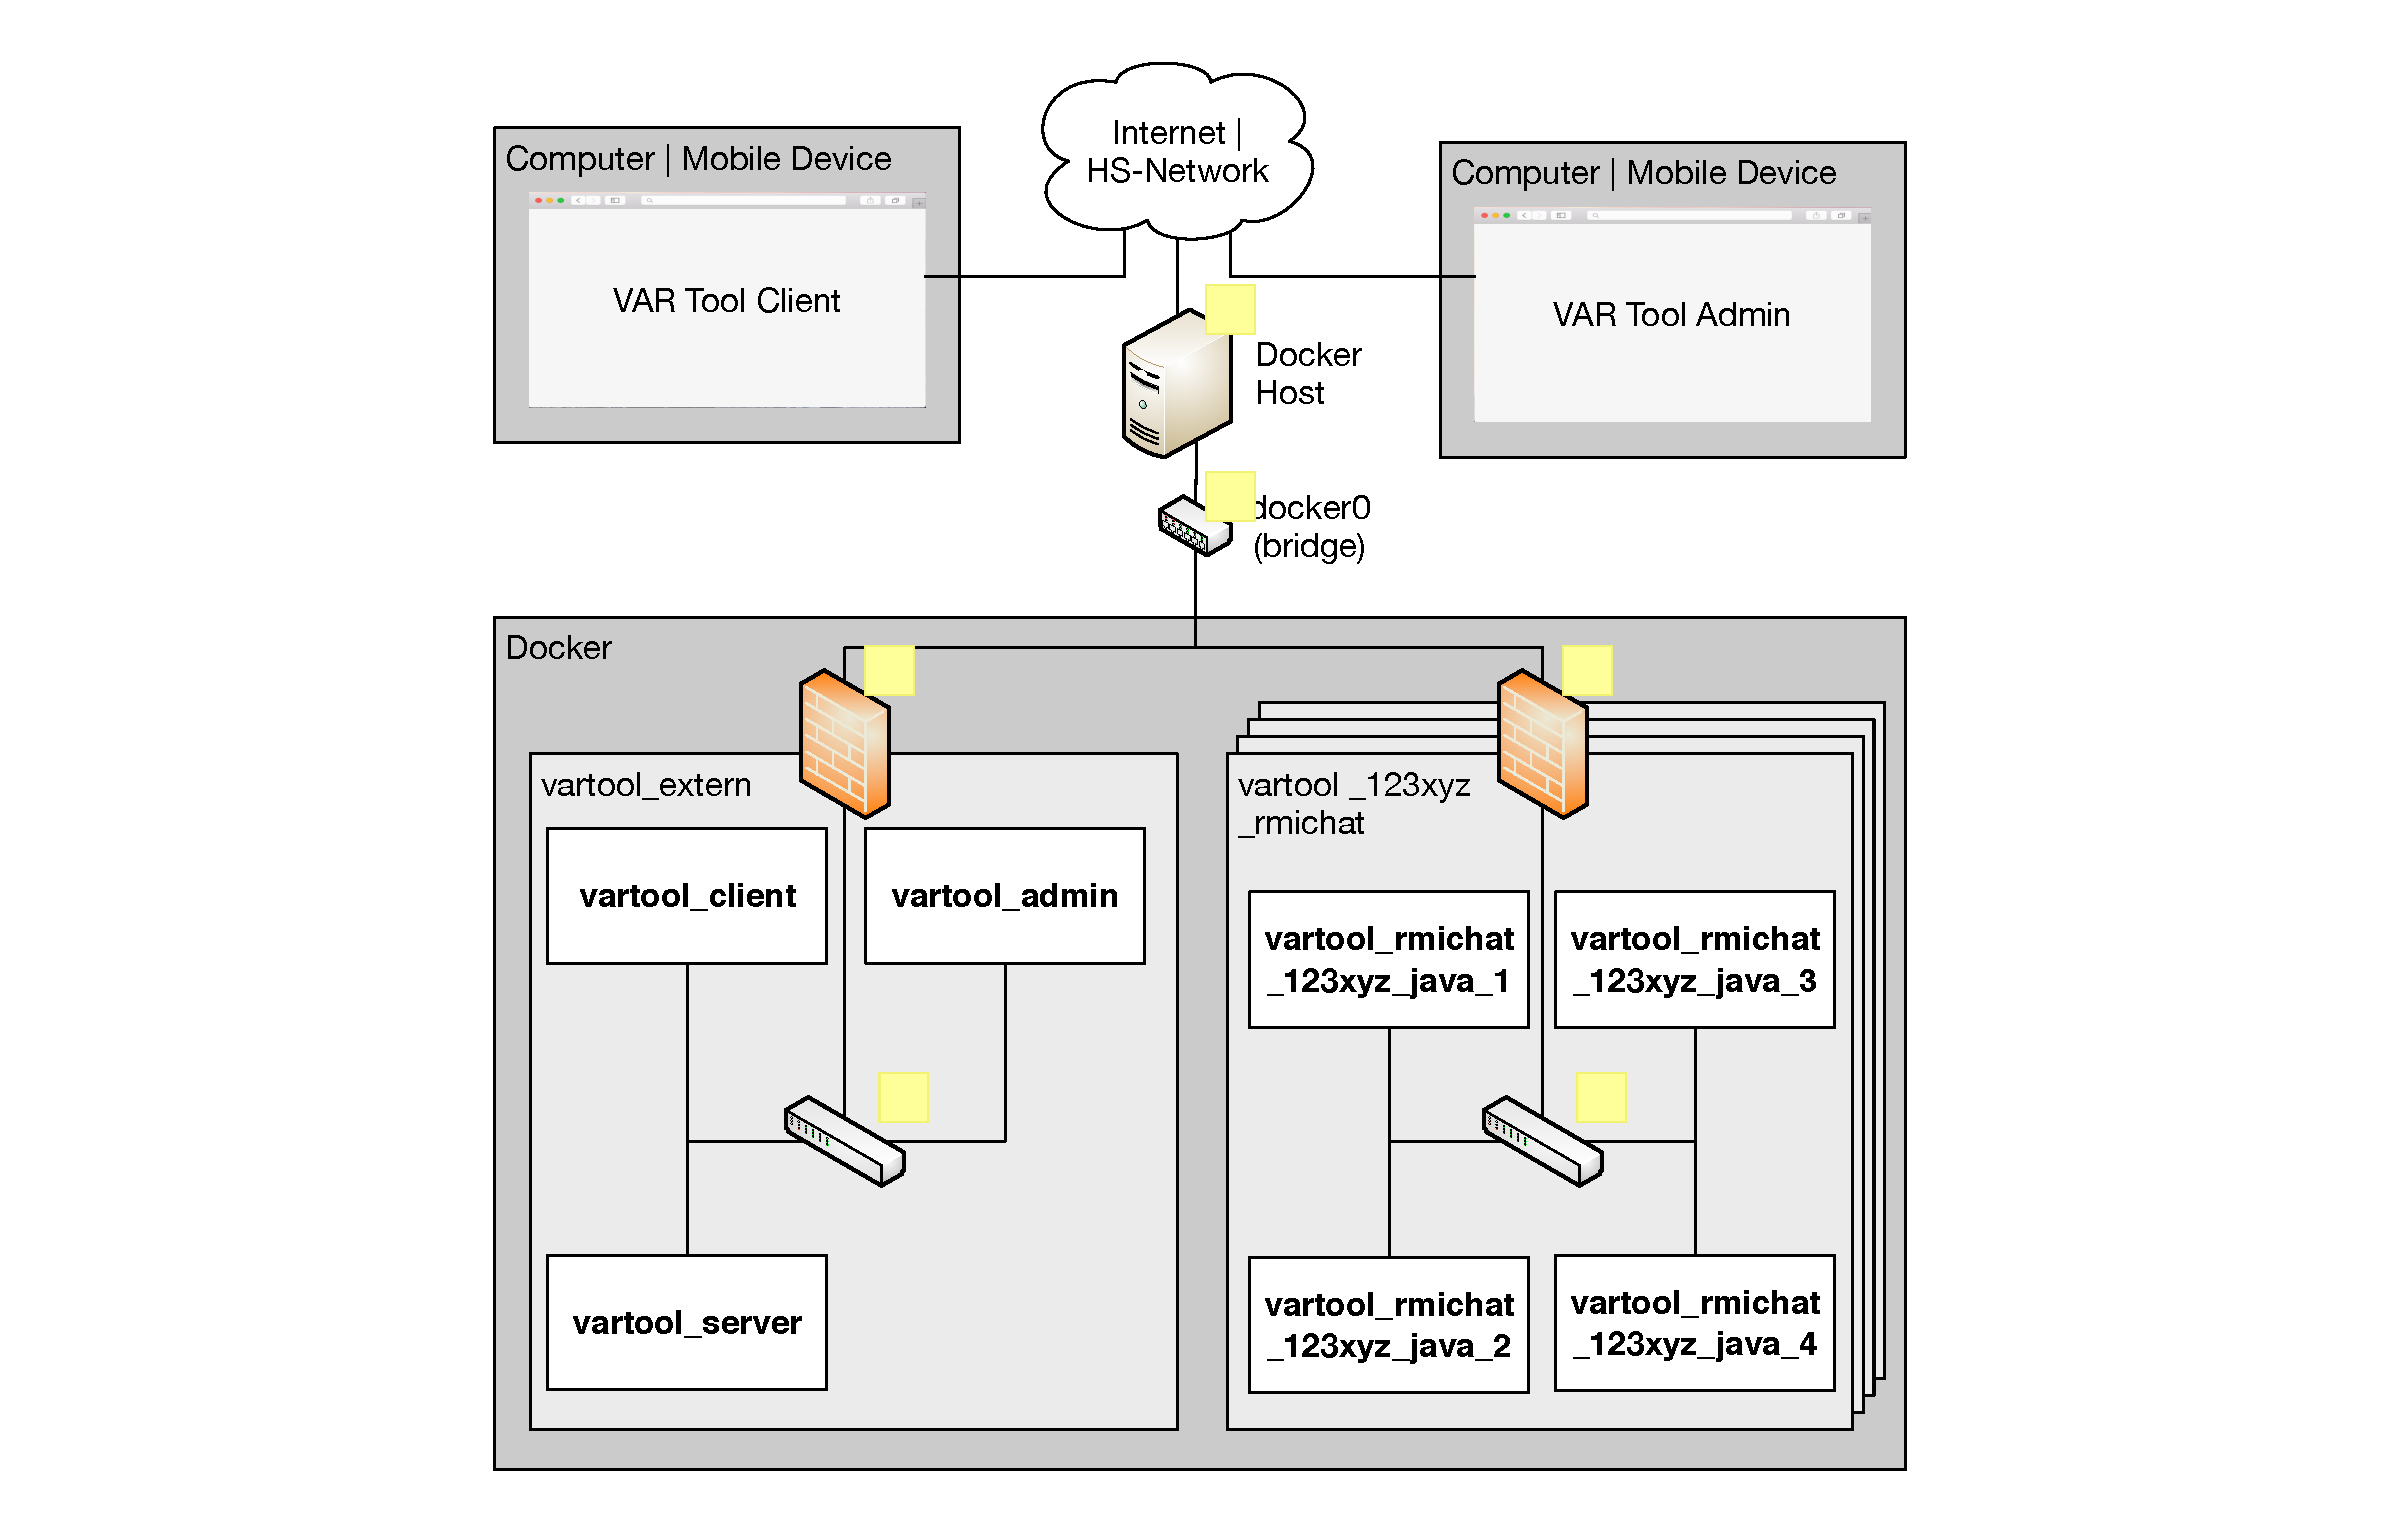
\includegraphics[width=\textwidth]{network_centered.pdf}
\end{frame}
\begin{frame}{State}
  \AddToShipoutPictureFG*{%
    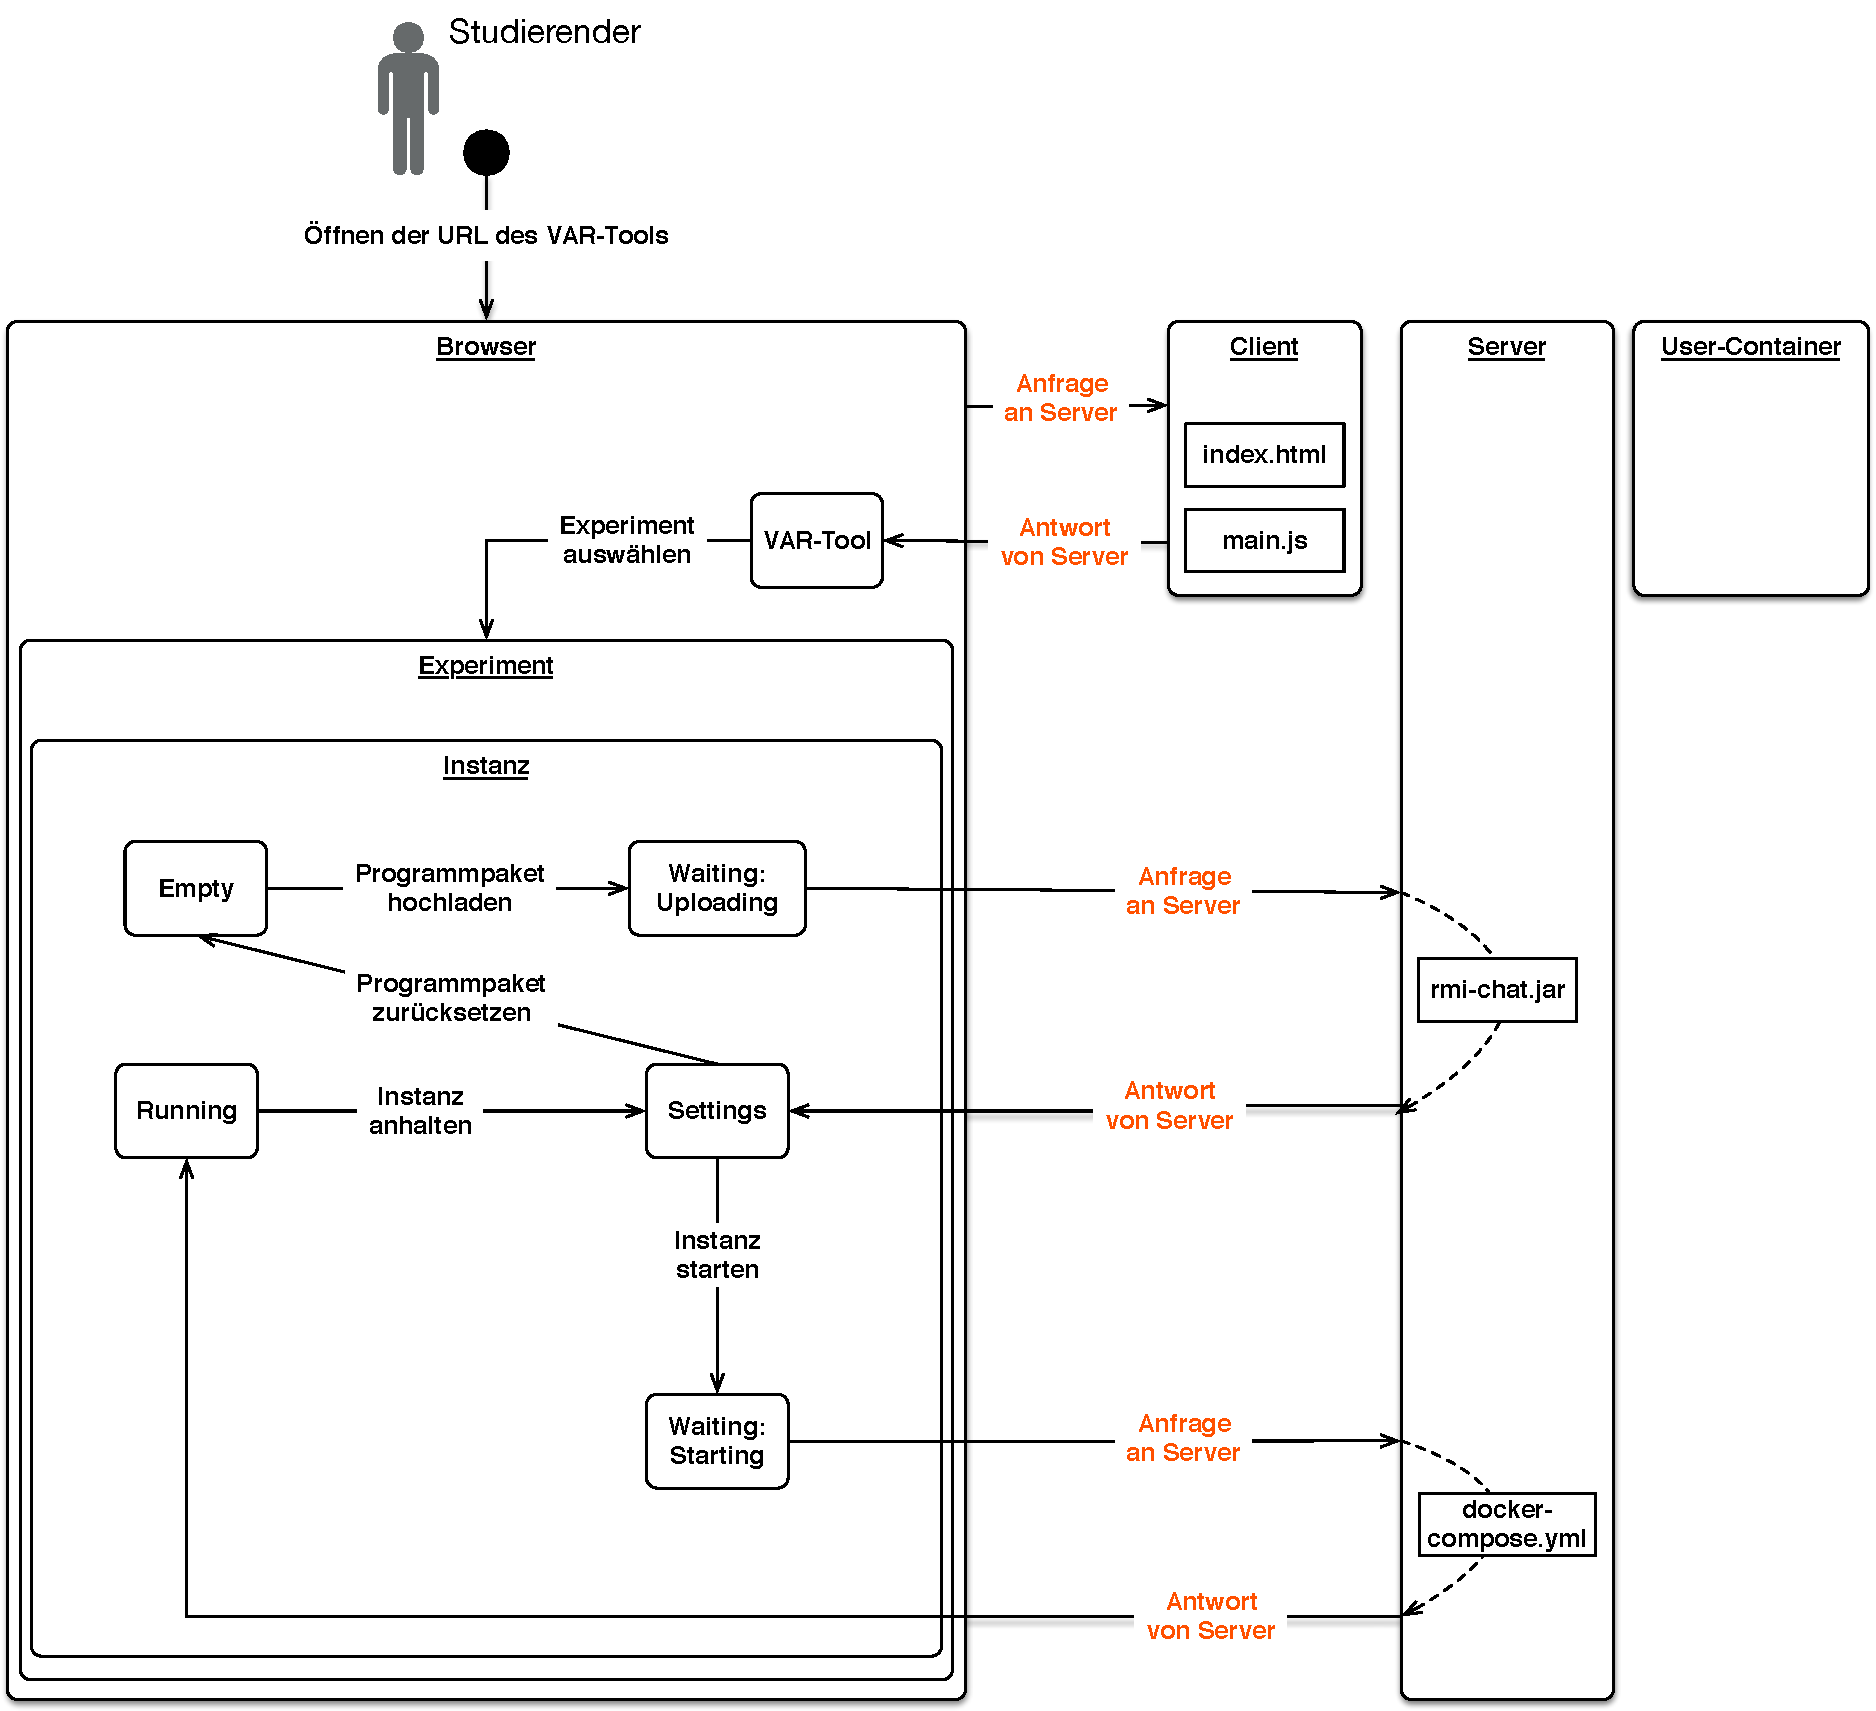
\includegraphics[width=\paperwidth,height=\textheight]{states.pdf}
  }
\end{frame}
\begin{frame}{Deployment}
  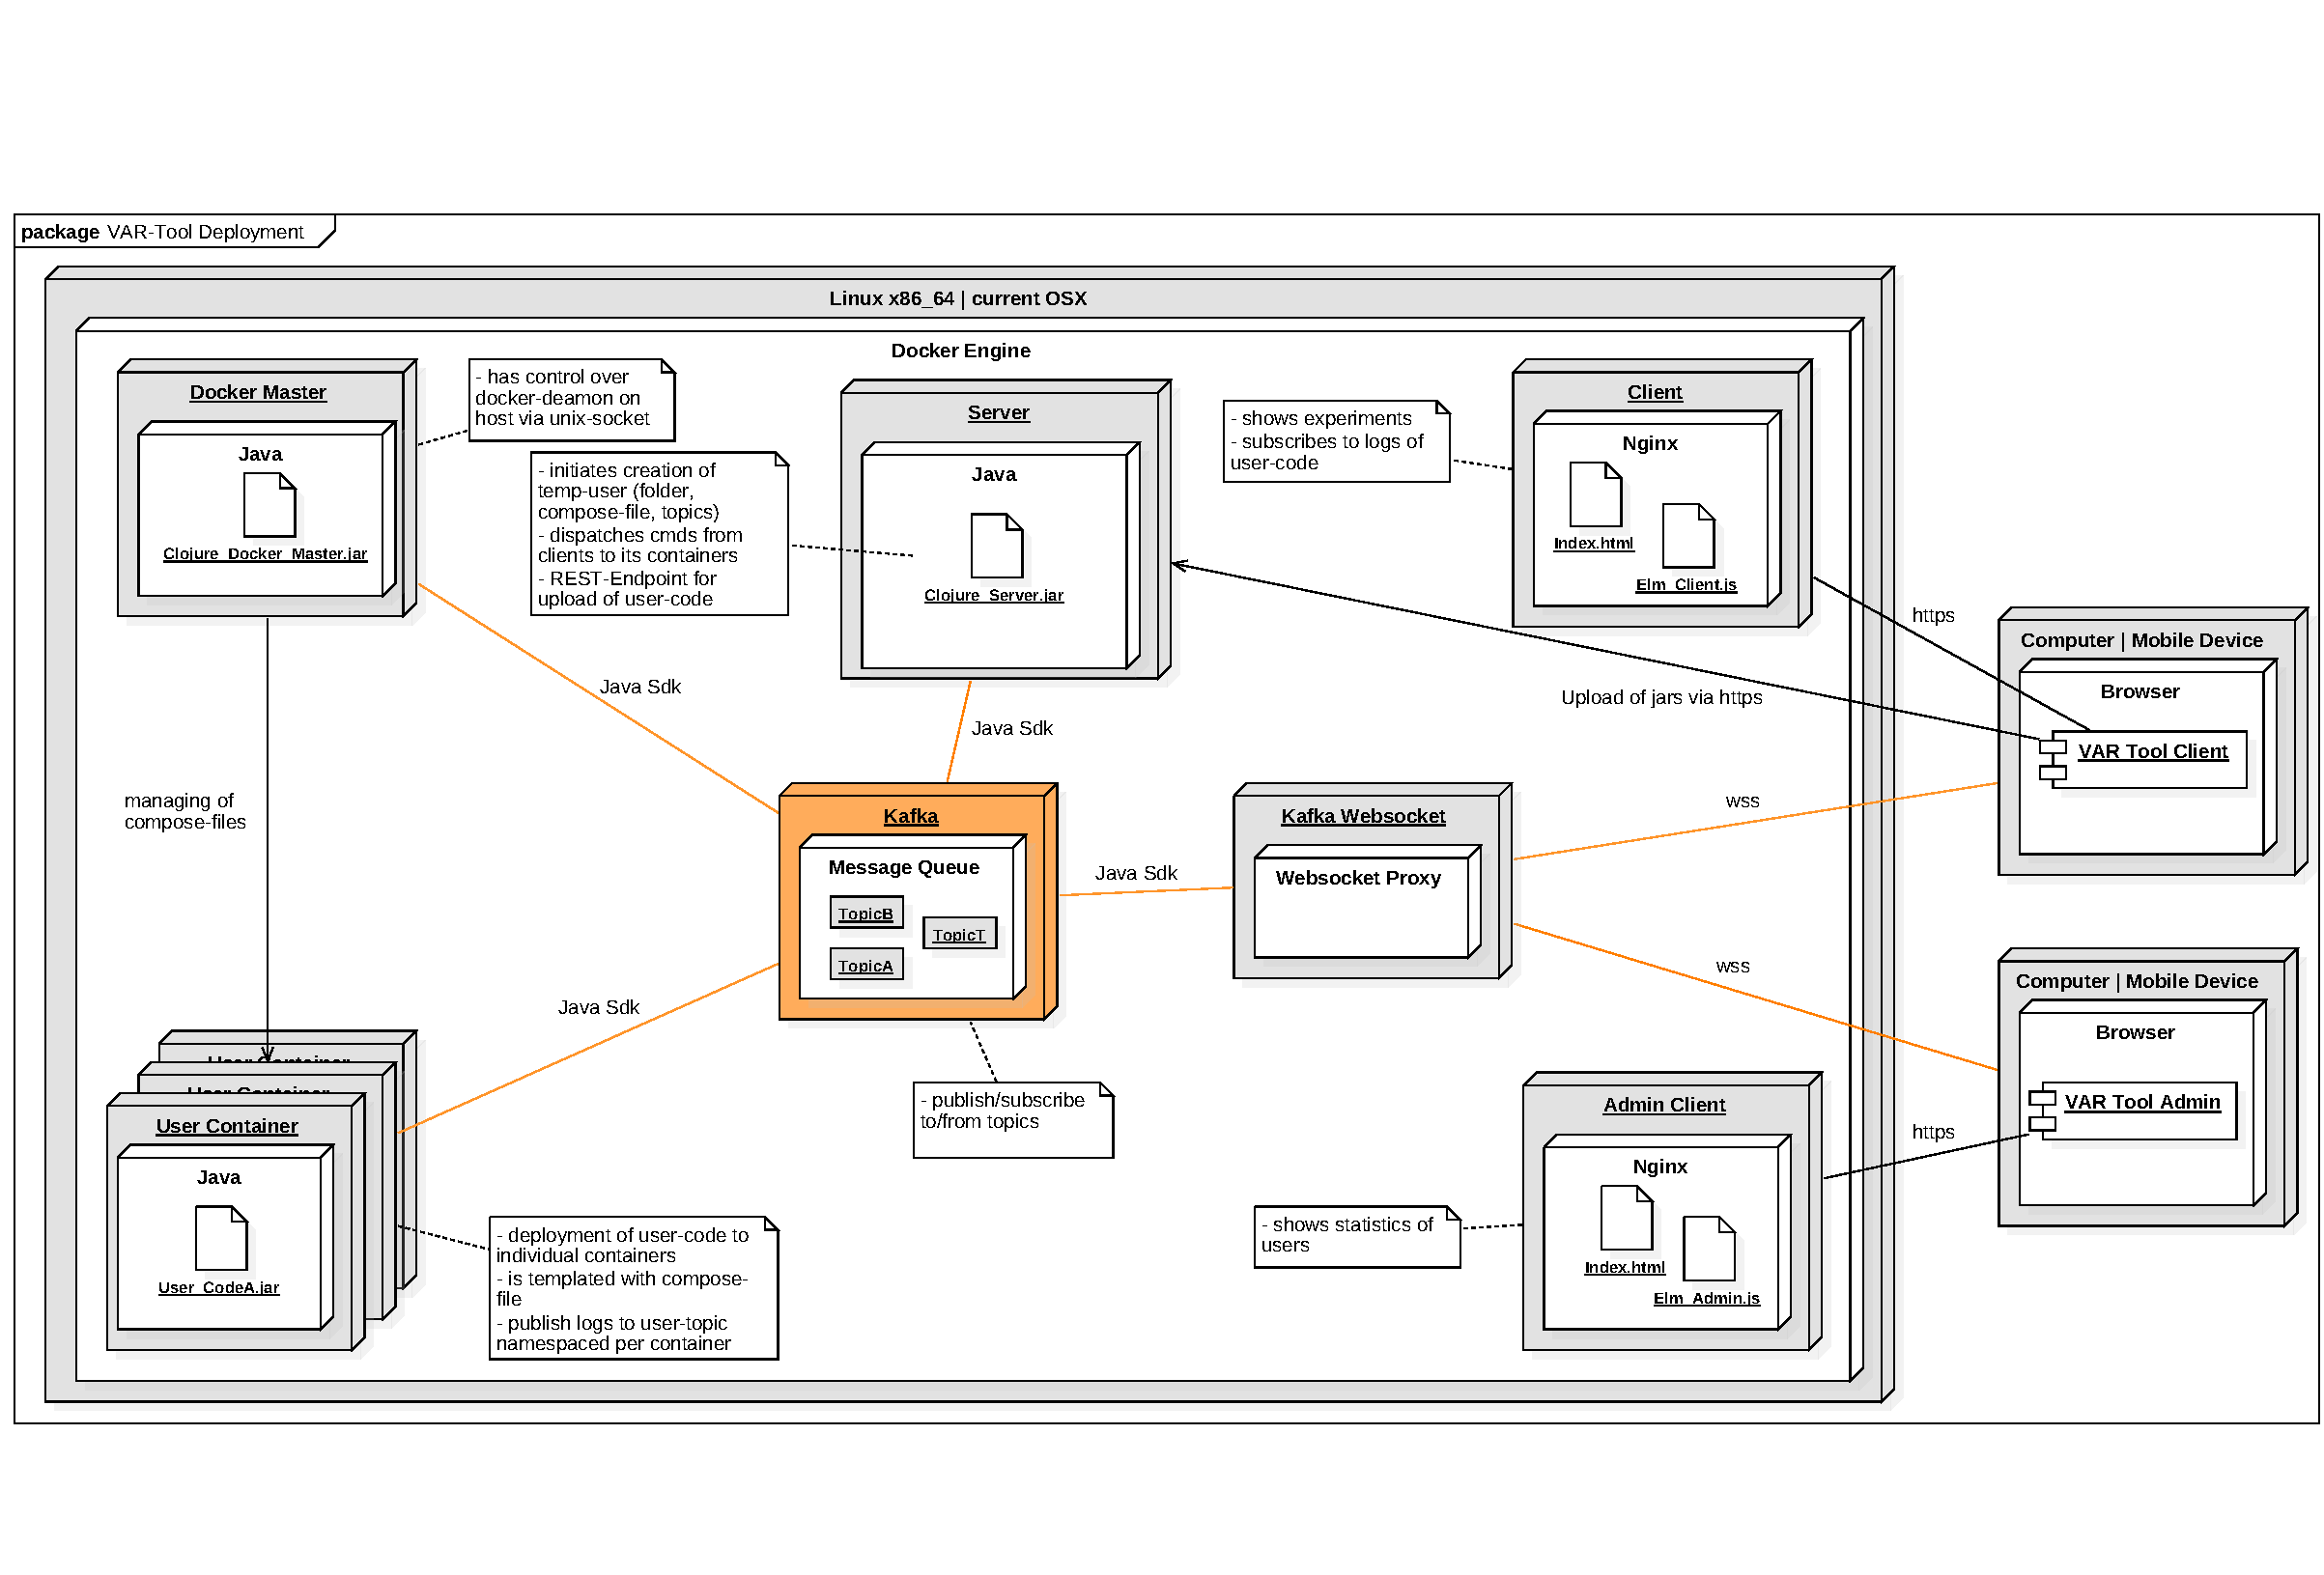
\includegraphics[width=\textwidth]{deployment.pdf}
\end{frame}
% \begin{frame}{Compose-File}
%   \AddToShipoutPictureFG*{%
%     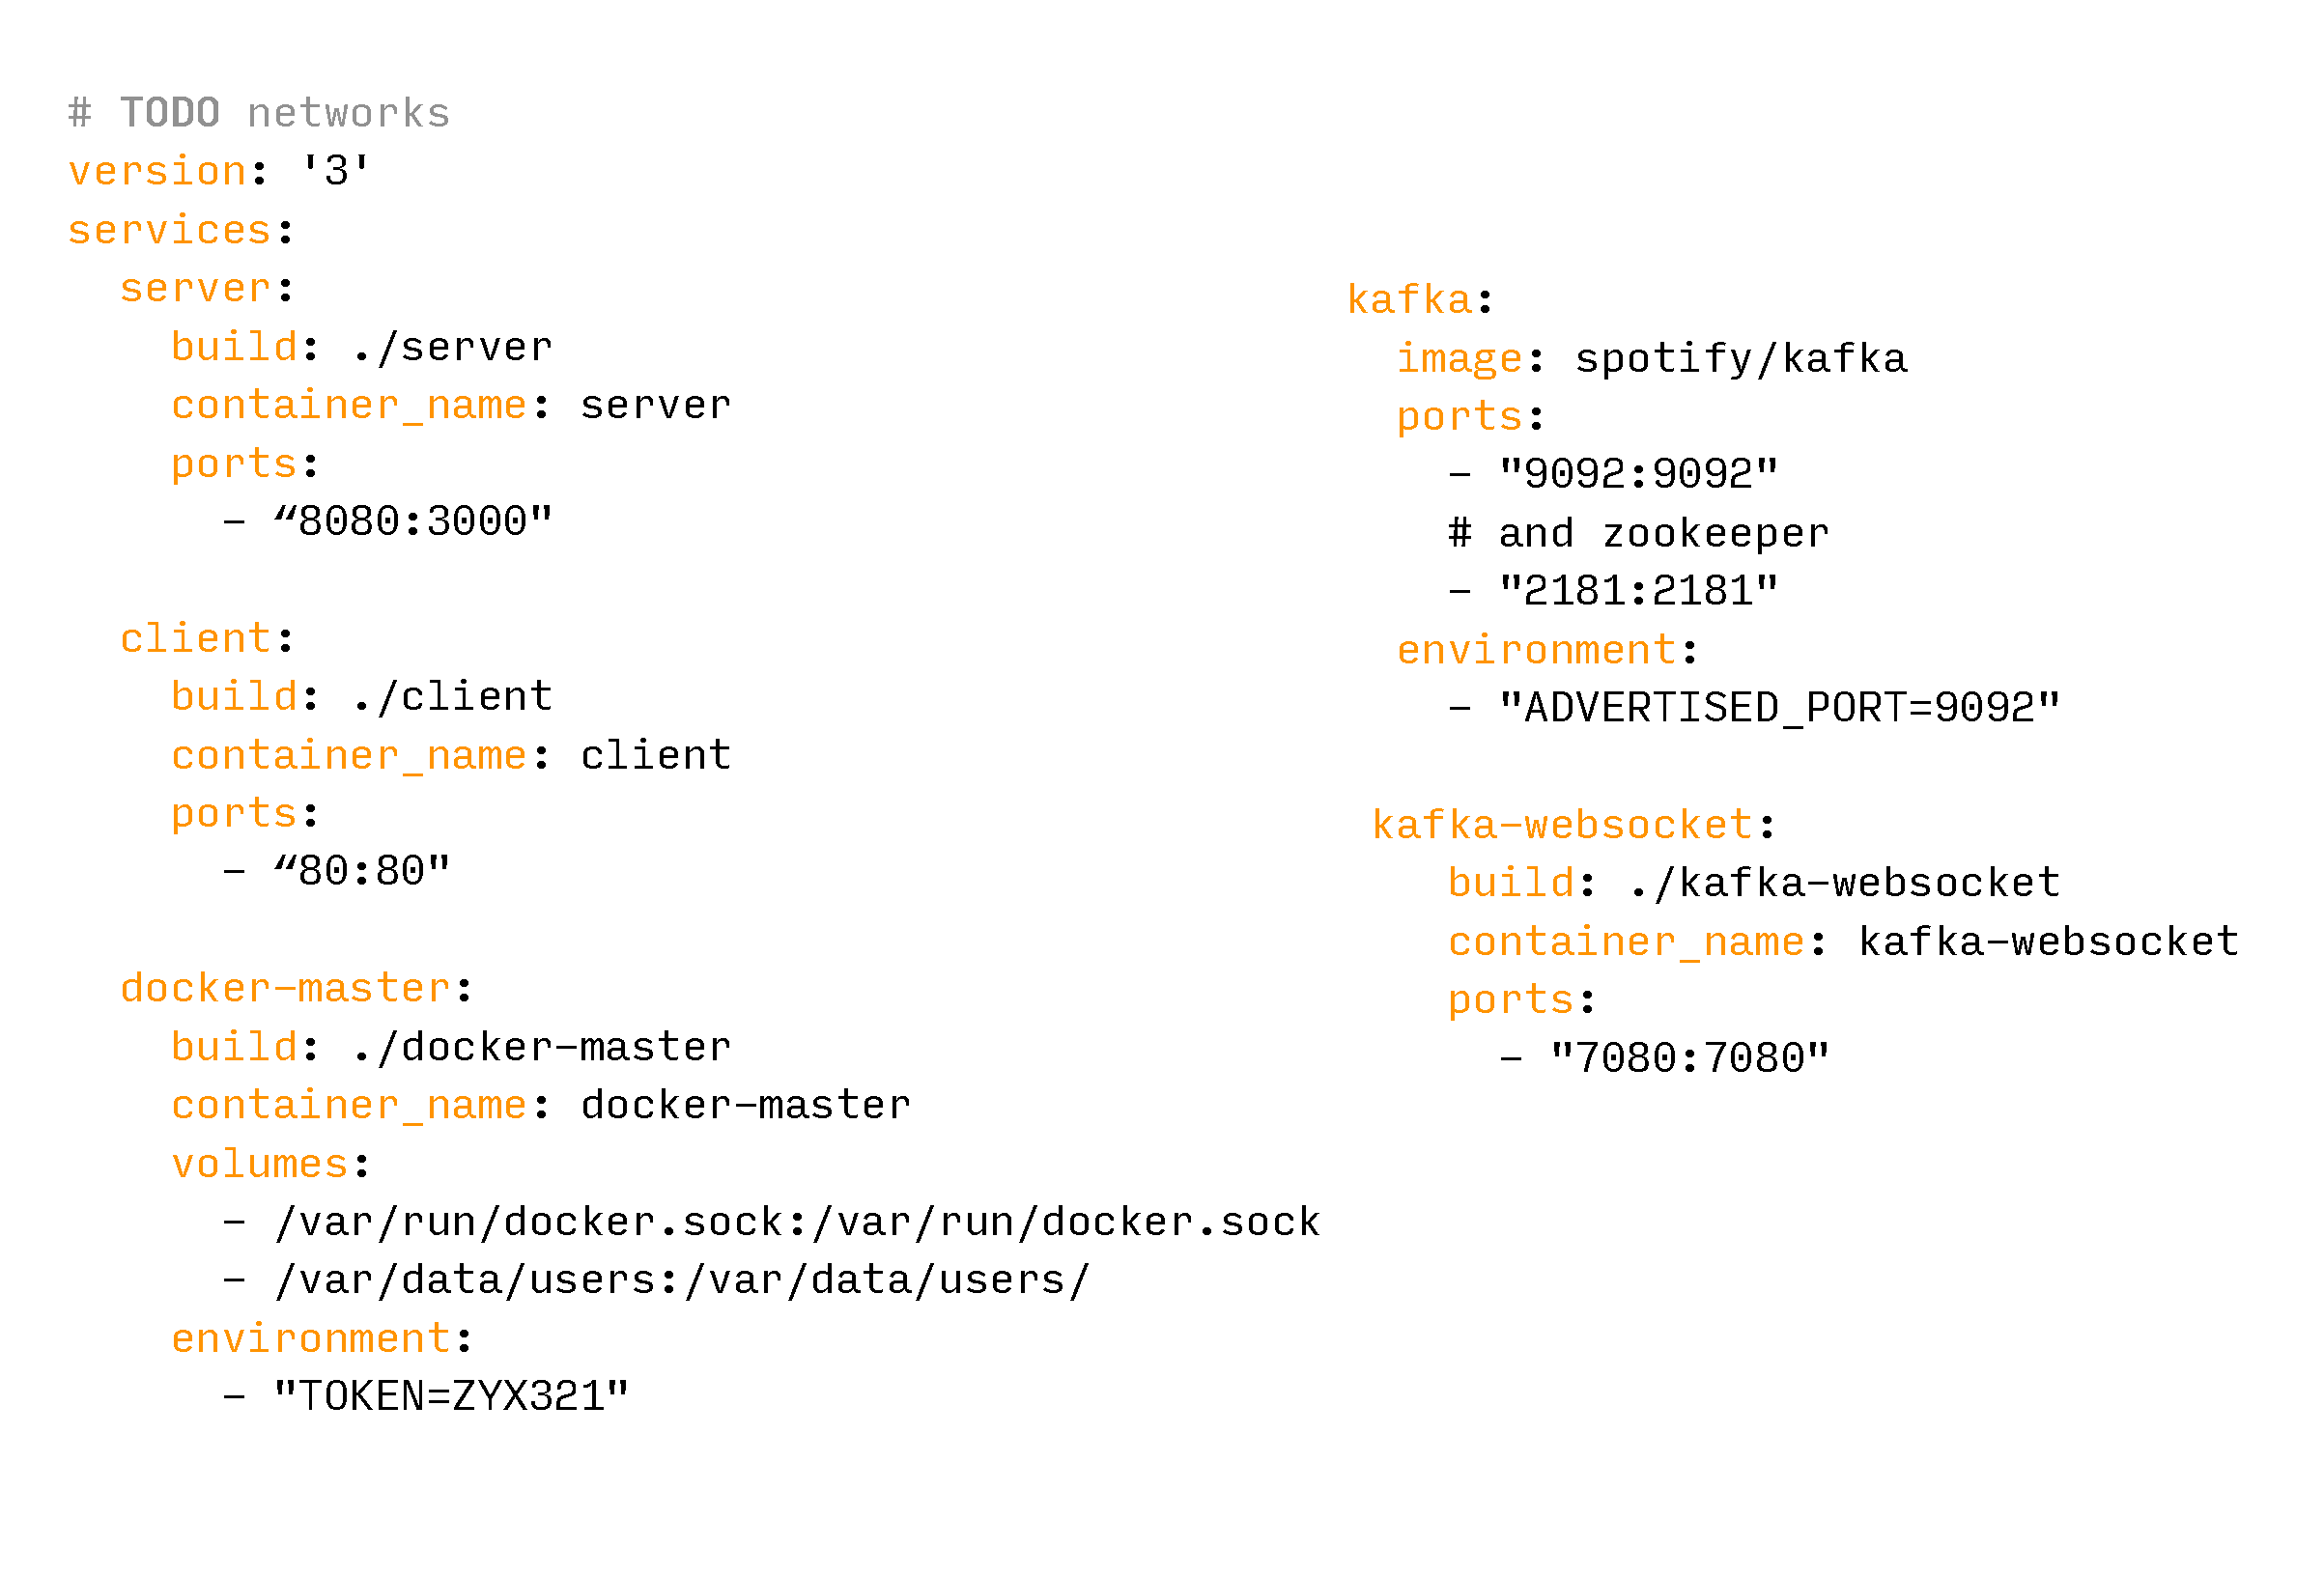
\includegraphics[width=\paperwidth,height=\textheight]{compose.pdf}
%   }
% \end{frame}

\section{Ausblick}
\begin{frame}{Fazit \& Ausblick}
  \begin{itemize}
    \item Docker in Docker // Binding von Docker-Socket\footnote{https://jpetazzo.github.io/2015/09/03/do-not-use-docker-in-docker-for-ci/}
  \end{itemize}
  \begin{itemize}
    \item Sehr spannendes Thema
    \item Viel Raum für weitere (studentische) Arbeiten
    \item Erstrebenswerte Aufgabe der Fakultät
  \end{itemize}
\end{frame}

% \begin{frame}[noframenumbering,plain]{Fin}
%   Danke für die Aufmerksamkeit. -- Fragen?
% \end{frame}
\end{document}
